\documentclass{book}
\usepackage[a4paper,top=2.5cm,bottom=2.5cm,left=2.5cm,right=2.5cm]{geometry}
\usepackage{makeidx}
\usepackage{natbib}
\usepackage{graphicx}
\usepackage{multicol}
\usepackage{float}
\usepackage{listings}
\usepackage{color}
\usepackage{ifthen}
\usepackage[table]{xcolor}
\usepackage{textcomp}
\usepackage{alltt}
\usepackage{ifpdf}
\ifpdf
\usepackage[pdftex,
            pagebackref=true,
            colorlinks=true,
            linkcolor=blue,
            unicode
           ]{hyperref}
\else
\usepackage[ps2pdf,
            pagebackref=true,
            colorlinks=true,
            linkcolor=blue,
            unicode
           ]{hyperref}
\usepackage{pspicture}
\fi
\usepackage[utf8]{inputenc}
\usepackage{mathptmx}
\usepackage[scaled=.90]{helvet}
\usepackage{courier}
\usepackage{sectsty}
\usepackage{amssymb}
\usepackage[titles]{tocloft}
\usepackage{doxygen}
\lstset{language=C++,inputencoding=utf8,basicstyle=\footnotesize,breaklines=true,breakatwhitespace=true,tabsize=4,numbers=left }
\makeindex
\setcounter{tocdepth}{3}
\renewcommand{\footrulewidth}{0.4pt}
\renewcommand{\familydefault}{\sfdefault}
\hfuzz=15pt
\setlength{\emergencystretch}{15pt}
\hbadness=750
\tolerance=750
\begin{document}
\hypersetup{pageanchor=false,citecolor=blue}
\begin{titlepage}
\vspace*{7cm}
\begin{center}
{\Large C\-S 242 Assignment 1.1 }\\
\vspace*{1cm}
{\large Generated by Doxygen 1.8.2}\\
\vspace*{0.5cm}
{\small Thu Sep 13 2012 14:30:10}\\
\end{center}
\end{titlepage}
\clearemptydoublepage
\pagenumbering{roman}
\tableofcontents
\clearemptydoublepage
\pagenumbering{arabic}
\hypersetup{pageanchor=true,citecolor=blue}
\chapter{Hierarchical Index}
\section{Class Hierarchy}
This inheritance list is sorted roughly, but not completely, alphabetically\-:\begin{DoxyCompactList}
\item \contentsline{section}{mazelib.\-tests.\-A\-Star\-Algorithm\-Test}{\pageref{classmazelib_1_1tests_1_1_a_star_algorithm_test}}{}
\item Comparable\begin{DoxyCompactList}
\item \contentsline{section}{mazelib.\-data.\-Node}{\pageref{classmazelib_1_1data_1_1_node}}{}
\end{DoxyCompactList}
\item \contentsline{section}{mazelib.\-tests.\-Dijkstras\-Algorithm\-Test}{\pageref{classmazelib_1_1tests_1_1_dijkstras_algorithm_test}}{}
\item \contentsline{section}{mazelib.\-data.\-Heuristic}{\pageref{interfacemazelib_1_1data_1_1_heuristic}}{}
\begin{DoxyCompactList}
\item \contentsline{section}{mazelib.\-data.\-Diagonal\-Distance}{\pageref{classmazelib_1_1data_1_1_diagonal_distance}}{}
\item \contentsline{section}{mazelib.\-data.\-Euclidean\-Distance}{\pageref{classmazelib_1_1data_1_1_euclidean_distance}}{}
\item \contentsline{section}{mazelib.\-data.\-Manhattan\-Distance}{\pageref{classmazelib_1_1data_1_1_manhattan_distance}}{}
\end{DoxyCompactList}
\item \contentsline{section}{mazelib.\-tests.\-Heuristics\-Test}{\pageref{classmazelib_1_1tests_1_1_heuristics_test}}{}
\item \contentsline{section}{mazelib.\-data.\-Maze}{\pageref{classmazelib_1_1data_1_1_maze}}{}
\item \contentsline{section}{mazelib.\-data.\-Maze\-Solver}{\pageref{classmazelib_1_1data_1_1_maze_solver}}{}
\begin{DoxyCompactList}
\item \contentsline{section}{mazelib.\-data.\-A\-Star\-Algorithm}{\pageref{classmazelib_1_1data_1_1_a_star_algorithm}}{}
\item \contentsline{section}{mazelib.\-data.\-Dijkstras\-Algorithm}{\pageref{classmazelib_1_1data_1_1_dijkstras_algorithm}}{}
\end{DoxyCompactList}
\item \contentsline{section}{mazelib.\-tests.\-Maze\-Test}{\pageref{classmazelib_1_1tests_1_1_maze_test}}{}
\item \contentsline{section}{mazelib.\-tests.\-Node\-Test}{\pageref{classmazelib_1_1tests_1_1_node_test}}{}
\item \contentsline{section}{mazelib.\-data.\-Position}{\pageref{classmazelib_1_1data_1_1_position}}{}
\item \contentsline{section}{mazelib.\-tests.\-Position\-Test}{\pageref{classmazelib_1_1tests_1_1_position_test}}{}
\end{DoxyCompactList}

\chapter{Class Index}
\section{Class List}
Here are the classes, structs, unions and interfaces with brief descriptions\-:\begin{DoxyCompactList}
\item\contentsline{section}{\hyperlink{classmazelib_1_1data_1_1_a_star_algorithm}{mazelib.\-data.\-A\-Star\-Algorithm} }{\pageref{classmazelib_1_1data_1_1_a_star_algorithm}}{}
\item\contentsline{section}{\hyperlink{classmazelib_1_1tests_1_1_a_star_algorithm_test}{mazelib.\-tests.\-A\-Star\-Algorithm\-Test} }{\pageref{classmazelib_1_1tests_1_1_a_star_algorithm_test}}{}
\item\contentsline{section}{\hyperlink{classmazelib_1_1data_1_1_diagonal_distance}{mazelib.\-data.\-Diagonal\-Distance} }{\pageref{classmazelib_1_1data_1_1_diagonal_distance}}{}
\item\contentsline{section}{\hyperlink{classmazelib_1_1data_1_1_dijkstras_algorithm}{mazelib.\-data.\-Dijkstras\-Algorithm} }{\pageref{classmazelib_1_1data_1_1_dijkstras_algorithm}}{}
\item\contentsline{section}{\hyperlink{classmazelib_1_1tests_1_1_dijkstras_algorithm_test}{mazelib.\-tests.\-Dijkstras\-Algorithm\-Test} }{\pageref{classmazelib_1_1tests_1_1_dijkstras_algorithm_test}}{}
\item\contentsline{section}{\hyperlink{classmazelib_1_1data_1_1_euclidean_distance}{mazelib.\-data.\-Euclidean\-Distance} }{\pageref{classmazelib_1_1data_1_1_euclidean_distance}}{}
\item\contentsline{section}{\hyperlink{interfacemazelib_1_1data_1_1_heuristic}{mazelib.\-data.\-Heuristic} }{\pageref{interfacemazelib_1_1data_1_1_heuristic}}{}
\item\contentsline{section}{\hyperlink{classmazelib_1_1tests_1_1_heuristics_test}{mazelib.\-tests.\-Heuristics\-Test} }{\pageref{classmazelib_1_1tests_1_1_heuristics_test}}{}
\item\contentsline{section}{\hyperlink{classmazelib_1_1data_1_1_manhattan_distance}{mazelib.\-data.\-Manhattan\-Distance} }{\pageref{classmazelib_1_1data_1_1_manhattan_distance}}{}
\item\contentsline{section}{\hyperlink{classmazelib_1_1data_1_1_maze}{mazelib.\-data.\-Maze} }{\pageref{classmazelib_1_1data_1_1_maze}}{}
\item\contentsline{section}{\hyperlink{classmazelib_1_1data_1_1_maze_solver}{mazelib.\-data.\-Maze\-Solver} }{\pageref{classmazelib_1_1data_1_1_maze_solver}}{}
\item\contentsline{section}{\hyperlink{classmazelib_1_1tests_1_1_maze_test}{mazelib.\-tests.\-Maze\-Test} }{\pageref{classmazelib_1_1tests_1_1_maze_test}}{}
\item\contentsline{section}{\hyperlink{classmazelib_1_1data_1_1_node}{mazelib.\-data.\-Node} }{\pageref{classmazelib_1_1data_1_1_node}}{}
\item\contentsline{section}{\hyperlink{classmazelib_1_1tests_1_1_node_test}{mazelib.\-tests.\-Node\-Test} }{\pageref{classmazelib_1_1tests_1_1_node_test}}{}
\item\contentsline{section}{\hyperlink{classmazelib_1_1data_1_1_position}{mazelib.\-data.\-Position} }{\pageref{classmazelib_1_1data_1_1_position}}{}
\item\contentsline{section}{\hyperlink{classmazelib_1_1tests_1_1_position_test}{mazelib.\-tests.\-Position\-Test} }{\pageref{classmazelib_1_1tests_1_1_position_test}}{}
\end{DoxyCompactList}

\chapter{Class Documentation}
\hypertarget{classmazelib_1_1data_1_1_a_star_algorithm}{\section{mazelib.\-data.\-A\-Star\-Algorithm Class Reference}
\label{classmazelib_1_1data_1_1_a_star_algorithm}\index{mazelib.\-data.\-A\-Star\-Algorithm@{mazelib.\-data.\-A\-Star\-Algorithm}}
}
Inheritance diagram for mazelib.\-data.\-A\-Star\-Algorithm\-:\begin{figure}[H]
\begin{center}
\leavevmode
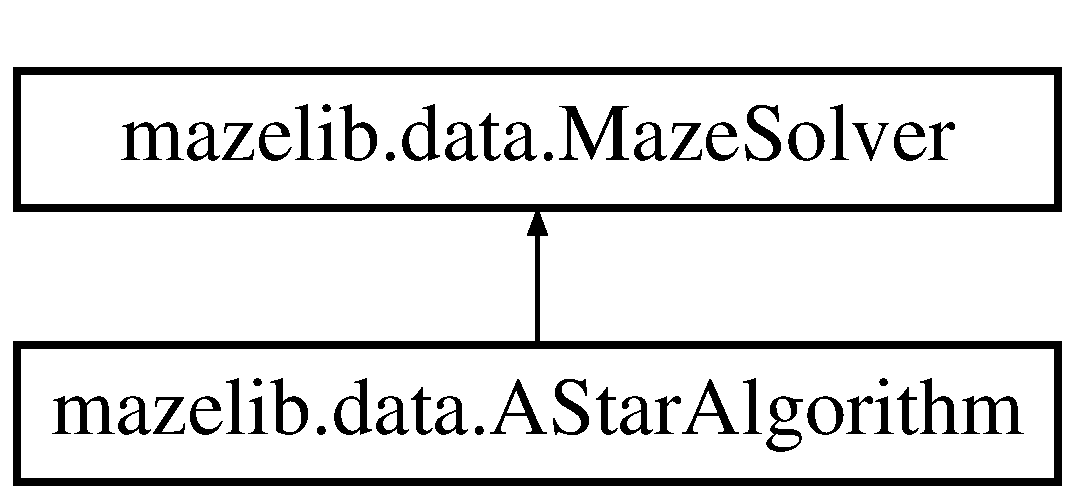
\includegraphics[height=2.000000cm]{classmazelib_1_1data_1_1_a_star_algorithm}
\end{center}
\end{figure}
\subsection*{Public Member Functions}
\begin{DoxyCompactItemize}
\item 
\hyperlink{classmazelib_1_1data_1_1_a_star_algorithm_af14ad7c669df46dd8c866223305a1f02}{A\-Star\-Algorithm} (\hyperlink{classmazelib_1_1data_1_1_maze}{Maze} maze, \hyperlink{interfacemazelib_1_1data_1_1_heuristic}{Heuristic} heuristic)
\item 
\hyperlink{classmazelib_1_1data_1_1_a_star_algorithm_a391f71803973c0d1241c5232dadee49f}{A\-Star\-Algorithm} (String string\-Maze, \hyperlink{interfacemazelib_1_1data_1_1_heuristic}{Heuristic} heuristic)
\item 
List$<$ \hyperlink{classmazelib_1_1data_1_1_node}{Node} $>$ \hyperlink{classmazelib_1_1data_1_1_a_star_algorithm_aaa690f9111cf47f54a10c84c28cfcba4}{solve\-Maze} ()
\end{DoxyCompactItemize}
\subsection*{Additional Inherited Members}


\subsection{Detailed Description}
\begin{DoxyAuthor}{Author}
Timur Reziapov \href{mailto:reziapo1@illinois.edu}{\tt reziapo1@illinois.\-edu} 
\end{DoxyAuthor}
\begin{DoxyDate}{Date}
Wednesday, September 5, 2012 15\-:00 P\-M 
\end{DoxyDate}


\subsection{Constructor \& Destructor Documentation}
\hypertarget{classmazelib_1_1data_1_1_a_star_algorithm_af14ad7c669df46dd8c866223305a1f02}{\index{mazelib\-::data\-::\-A\-Star\-Algorithm@{mazelib\-::data\-::\-A\-Star\-Algorithm}!A\-Star\-Algorithm@{A\-Star\-Algorithm}}
\index{A\-Star\-Algorithm@{A\-Star\-Algorithm}!mazelib::data::AStarAlgorithm@{mazelib\-::data\-::\-A\-Star\-Algorithm}}
\subsubsection[{A\-Star\-Algorithm}]{\setlength{\rightskip}{0pt plus 5cm}mazelib.\-data.\-A\-Star\-Algorithm.\-A\-Star\-Algorithm (
\begin{DoxyParamCaption}
\item[{{\bf Maze}}]{maze, }
\item[{{\bf Heuristic}}]{heuristic}
\end{DoxyParamCaption}
)\hspace{0.3cm}{\ttfamily [inline]}}}\label{classmazelib_1_1data_1_1_a_star_algorithm_af14ad7c669df46dd8c866223305a1f02}
Constructor for A\-Star\-Agorithm Object. 
\begin{DoxyParams}{Parameters}
{\em maze} & the \hyperlink{classmazelib_1_1data_1_1_maze}{Maze} to solve \\
\hline
\end{DoxyParams}
\hypertarget{classmazelib_1_1data_1_1_a_star_algorithm_a391f71803973c0d1241c5232dadee49f}{\index{mazelib\-::data\-::\-A\-Star\-Algorithm@{mazelib\-::data\-::\-A\-Star\-Algorithm}!A\-Star\-Algorithm@{A\-Star\-Algorithm}}
\index{A\-Star\-Algorithm@{A\-Star\-Algorithm}!mazelib::data::AStarAlgorithm@{mazelib\-::data\-::\-A\-Star\-Algorithm}}
\subsubsection[{A\-Star\-Algorithm}]{\setlength{\rightskip}{0pt plus 5cm}mazelib.\-data.\-A\-Star\-Algorithm.\-A\-Star\-Algorithm (
\begin{DoxyParamCaption}
\item[{String}]{string\-Maze, }
\item[{{\bf Heuristic}}]{heuristic}
\end{DoxyParamCaption}
)\hspace{0.3cm}{\ttfamily [inline]}}}\label{classmazelib_1_1data_1_1_a_star_algorithm_a391f71803973c0d1241c5232dadee49f}
Constructor for A\-Star\-Agorithm Object. 
\begin{DoxyParams}{Parameters}
{\em string\-Maze} & the string representation of the \hyperlink{classmazelib_1_1data_1_1_maze}{Maze} to solve \\
\hline
\end{DoxyParams}


\subsection{Member Function Documentation}
\hypertarget{classmazelib_1_1data_1_1_a_star_algorithm_aaa690f9111cf47f54a10c84c28cfcba4}{\index{mazelib\-::data\-::\-A\-Star\-Algorithm@{mazelib\-::data\-::\-A\-Star\-Algorithm}!solve\-Maze@{solve\-Maze}}
\index{solve\-Maze@{solve\-Maze}!mazelib::data::AStarAlgorithm@{mazelib\-::data\-::\-A\-Star\-Algorithm}}
\subsubsection[{solve\-Maze}]{\setlength{\rightskip}{0pt plus 5cm}List$<${\bf Node}$>$ mazelib.\-data.\-A\-Star\-Algorithm.\-solve\-Maze (
\begin{DoxyParamCaption}
{}
\end{DoxyParamCaption}
)\hspace{0.3cm}{\ttfamily [inline]}, {\ttfamily [virtual]}}}\label{classmazelib_1_1data_1_1_a_star_algorithm_aaa690f9111cf47f54a10c84c28cfcba4}
The main function of the algorithm. \begin{DoxyReturn}{Returns}
List of Nodes that represent the solution to this maze, null if there is no path from start \hyperlink{classmazelib_1_1data_1_1_node}{Node} to end \hyperlink{classmazelib_1_1data_1_1_node}{Node} 
\end{DoxyReturn}


Implements \hyperlink{classmazelib_1_1data_1_1_maze_solver_a009bd983cdccfb7c845d3da8fabf02d6}{mazelib.\-data.\-Maze\-Solver}.



The documentation for this class was generated from the following file\-:\begin{DoxyCompactItemize}
\item 
src/mazelib/data/A\-Star\-Algorithm.\-java\end{DoxyCompactItemize}

\hypertarget{classmazelib_1_1tests_1_1_a_star_algorithm_test}{\section{mazelib.\-tests.\-A\-Star\-Algorithm\-Test Class Reference}
\label{classmazelib_1_1tests_1_1_a_star_algorithm_test}\index{mazelib.\-tests.\-A\-Star\-Algorithm\-Test@{mazelib.\-tests.\-A\-Star\-Algorithm\-Test}}
}
\subsection*{Public Member Functions}
\begin{DoxyCompactItemize}
\item 
void \hyperlink{classmazelib_1_1tests_1_1_a_star_algorithm_test_aec72fa33496b078a0ee88787b17a7cc5}{test\-Initialization} ()
\item 
void \hyperlink{classmazelib_1_1tests_1_1_a_star_algorithm_test_ad9fcdd615a22dabd3bb98b1b81dc530e}{test\-Main\-Exceptions} ()
\item 
void \hyperlink{classmazelib_1_1tests_1_1_a_star_algorithm_test_afa88278c8a99dc756060007a71298d2f}{test\-Open\-Area} ()
\item 
void \hyperlink{classmazelib_1_1tests_1_1_a_star_algorithm_test_a07d1b247735c9e93be964c1586f55429}{test\-Wall} ()
\item 
void \hyperlink{classmazelib_1_1tests_1_1_a_star_algorithm_test_a70d4c1c704f663de17dd29062f923277}{test\-Wall\-Bottom} ()
\item 
void \hyperlink{classmazelib_1_1tests_1_1_a_star_algorithm_test_a04e1e2fc7c9f096b47e0020ecefce31f}{test\-Choose\-Shortest\-Path} ()
\item 
void \hyperlink{classmazelib_1_1tests_1_1_a_star_algorithm_test_af211b27410c2c9b99f7d4ada33cf73d1}{test\-Big\-Maze} ()
\item 
void \hyperlink{classmazelib_1_1tests_1_1_a_star_algorithm_test_a1fe74aadca4426101c6b37bad8c3bcc1}{test\-Unsolvable} ()
\item 
void \hyperlink{classmazelib_1_1tests_1_1_a_star_algorithm_test_a1dff79da0548389e66dafcbe2cd5cbbe}{test\-Unsolvable\-Diagonal} ()
\item 
void \hyperlink{classmazelib_1_1tests_1_1_a_star_algorithm_test_a947f5b9044e94187fe46787c388df05b}{test\-Heuristic\-Independence} ()
\item 
void \hyperlink{classmazelib_1_1tests_1_1_a_star_algorithm_test_a0ef8a993413de21e3ded9372183d637d}{test\-Draw\-Solution} ()
\end{DoxyCompactItemize}


\subsection{Detailed Description}
\begin{DoxyAuthor}{Author}
Timur Reziapov \href{mailto:reziapo1@illinois.edu}{\tt reziapo1@illinois.\-edu} 
\end{DoxyAuthor}
\begin{DoxyDate}{Date}
Tuesday, September 4, 2012, 18\-:00 P\-M 
\end{DoxyDate}


\subsection{Member Function Documentation}
\hypertarget{classmazelib_1_1tests_1_1_a_star_algorithm_test_af211b27410c2c9b99f7d4ada33cf73d1}{\index{mazelib\-::tests\-::\-A\-Star\-Algorithm\-Test@{mazelib\-::tests\-::\-A\-Star\-Algorithm\-Test}!test\-Big\-Maze@{test\-Big\-Maze}}
\index{test\-Big\-Maze@{test\-Big\-Maze}!mazelib::tests::AStarAlgorithmTest@{mazelib\-::tests\-::\-A\-Star\-Algorithm\-Test}}
\subsubsection[{test\-Big\-Maze}]{\setlength{\rightskip}{0pt plus 5cm}void mazelib.\-tests.\-A\-Star\-Algorithm\-Test.\-test\-Big\-Maze (
\begin{DoxyParamCaption}
{}
\end{DoxyParamCaption}
)\hspace{0.3cm}{\ttfamily [inline]}}}\label{classmazelib_1_1tests_1_1_a_star_algorithm_test_af211b27410c2c9b99f7d4ada33cf73d1}
This test checks if the algorithm can solve relatively big Mazes. \hypertarget{classmazelib_1_1tests_1_1_a_star_algorithm_test_a04e1e2fc7c9f096b47e0020ecefce31f}{\index{mazelib\-::tests\-::\-A\-Star\-Algorithm\-Test@{mazelib\-::tests\-::\-A\-Star\-Algorithm\-Test}!test\-Choose\-Shortest\-Path@{test\-Choose\-Shortest\-Path}}
\index{test\-Choose\-Shortest\-Path@{test\-Choose\-Shortest\-Path}!mazelib::tests::AStarAlgorithmTest@{mazelib\-::tests\-::\-A\-Star\-Algorithm\-Test}}
\subsubsection[{test\-Choose\-Shortest\-Path}]{\setlength{\rightskip}{0pt plus 5cm}void mazelib.\-tests.\-A\-Star\-Algorithm\-Test.\-test\-Choose\-Shortest\-Path (
\begin{DoxyParamCaption}
{}
\end{DoxyParamCaption}
)\hspace{0.3cm}{\ttfamily [inline]}}}\label{classmazelib_1_1tests_1_1_a_star_algorithm_test_a04e1e2fc7c9f096b47e0020ecefce31f}
This test checks if solver chooses the shortest path when there are multiple paths leading to the end Node. Shortest path is the one with most diagonal moves. \hypertarget{classmazelib_1_1tests_1_1_a_star_algorithm_test_a0ef8a993413de21e3ded9372183d637d}{\index{mazelib\-::tests\-::\-A\-Star\-Algorithm\-Test@{mazelib\-::tests\-::\-A\-Star\-Algorithm\-Test}!test\-Draw\-Solution@{test\-Draw\-Solution}}
\index{test\-Draw\-Solution@{test\-Draw\-Solution}!mazelib::tests::AStarAlgorithmTest@{mazelib\-::tests\-::\-A\-Star\-Algorithm\-Test}}
\subsubsection[{test\-Draw\-Solution}]{\setlength{\rightskip}{0pt plus 5cm}void mazelib.\-tests.\-A\-Star\-Algorithm\-Test.\-test\-Draw\-Solution (
\begin{DoxyParamCaption}
{}
\end{DoxyParamCaption}
)\hspace{0.3cm}{\ttfamily [inline]}}}\label{classmazelib_1_1tests_1_1_a_star_algorithm_test_a0ef8a993413de21e3ded9372183d637d}
This test checks if draw\-Solutiion returns the same output if called twice and returns a String representation of successfully solved maze. \hypertarget{classmazelib_1_1tests_1_1_a_star_algorithm_test_a947f5b9044e94187fe46787c388df05b}{\index{mazelib\-::tests\-::\-A\-Star\-Algorithm\-Test@{mazelib\-::tests\-::\-A\-Star\-Algorithm\-Test}!test\-Heuristic\-Independence@{test\-Heuristic\-Independence}}
\index{test\-Heuristic\-Independence@{test\-Heuristic\-Independence}!mazelib::tests::AStarAlgorithmTest@{mazelib\-::tests\-::\-A\-Star\-Algorithm\-Test}}
\subsubsection[{test\-Heuristic\-Independence}]{\setlength{\rightskip}{0pt plus 5cm}void mazelib.\-tests.\-A\-Star\-Algorithm\-Test.\-test\-Heuristic\-Independence (
\begin{DoxyParamCaption}
{}
\end{DoxyParamCaption}
)\hspace{0.3cm}{\ttfamily [inline]}}}\label{classmazelib_1_1tests_1_1_a_star_algorithm_test_a947f5b9044e94187fe46787c388df05b}
This test checks if Mazes are solveable regardless of the Heuristic used. \hypertarget{classmazelib_1_1tests_1_1_a_star_algorithm_test_aec72fa33496b078a0ee88787b17a7cc5}{\index{mazelib\-::tests\-::\-A\-Star\-Algorithm\-Test@{mazelib\-::tests\-::\-A\-Star\-Algorithm\-Test}!test\-Initialization@{test\-Initialization}}
\index{test\-Initialization@{test\-Initialization}!mazelib::tests::AStarAlgorithmTest@{mazelib\-::tests\-::\-A\-Star\-Algorithm\-Test}}
\subsubsection[{test\-Initialization}]{\setlength{\rightskip}{0pt plus 5cm}void mazelib.\-tests.\-A\-Star\-Algorithm\-Test.\-test\-Initialization (
\begin{DoxyParamCaption}
{}
\end{DoxyParamCaption}
)\hspace{0.3cm}{\ttfamily [inline]}}}\label{classmazelib_1_1tests_1_1_a_star_algorithm_test_aec72fa33496b078a0ee88787b17a7cc5}
Test to check A\-Start\-Algorithm object initialization. Checks both Maze and String constructors. \hypertarget{classmazelib_1_1tests_1_1_a_star_algorithm_test_ad9fcdd615a22dabd3bb98b1b81dc530e}{\index{mazelib\-::tests\-::\-A\-Star\-Algorithm\-Test@{mazelib\-::tests\-::\-A\-Star\-Algorithm\-Test}!test\-Main\-Exceptions@{test\-Main\-Exceptions}}
\index{test\-Main\-Exceptions@{test\-Main\-Exceptions}!mazelib::tests::AStarAlgorithmTest@{mazelib\-::tests\-::\-A\-Star\-Algorithm\-Test}}
\subsubsection[{test\-Main\-Exceptions}]{\setlength{\rightskip}{0pt plus 5cm}void mazelib.\-tests.\-A\-Star\-Algorithm\-Test.\-test\-Main\-Exceptions (
\begin{DoxyParamCaption}
{}
\end{DoxyParamCaption}
)\hspace{0.3cm}{\ttfamily [inline]}}}\label{classmazelib_1_1tests_1_1_a_star_algorithm_test_ad9fcdd615a22dabd3bb98b1b81dc530e}
Test to check if main function causes any exceptions. \hypertarget{classmazelib_1_1tests_1_1_a_star_algorithm_test_afa88278c8a99dc756060007a71298d2f}{\index{mazelib\-::tests\-::\-A\-Star\-Algorithm\-Test@{mazelib\-::tests\-::\-A\-Star\-Algorithm\-Test}!test\-Open\-Area@{test\-Open\-Area}}
\index{test\-Open\-Area@{test\-Open\-Area}!mazelib::tests::AStarAlgorithmTest@{mazelib\-::tests\-::\-A\-Star\-Algorithm\-Test}}
\subsubsection[{test\-Open\-Area}]{\setlength{\rightskip}{0pt plus 5cm}void mazelib.\-tests.\-A\-Star\-Algorithm\-Test.\-test\-Open\-Area (
\begin{DoxyParamCaption}
{}
\end{DoxyParamCaption}
)\hspace{0.3cm}{\ttfamily [inline]}}}\label{classmazelib_1_1tests_1_1_a_star_algorithm_test_afa88278c8a99dc756060007a71298d2f}
This test checks if the algorithm can find a way in an area with no walls. \hypertarget{classmazelib_1_1tests_1_1_a_star_algorithm_test_a1fe74aadca4426101c6b37bad8c3bcc1}{\index{mazelib\-::tests\-::\-A\-Star\-Algorithm\-Test@{mazelib\-::tests\-::\-A\-Star\-Algorithm\-Test}!test\-Unsolvable@{test\-Unsolvable}}
\index{test\-Unsolvable@{test\-Unsolvable}!mazelib::tests::AStarAlgorithmTest@{mazelib\-::tests\-::\-A\-Star\-Algorithm\-Test}}
\subsubsection[{test\-Unsolvable}]{\setlength{\rightskip}{0pt plus 5cm}void mazelib.\-tests.\-A\-Star\-Algorithm\-Test.\-test\-Unsolvable (
\begin{DoxyParamCaption}
{}
\end{DoxyParamCaption}
)\hspace{0.3cm}{\ttfamily [inline]}}}\label{classmazelib_1_1tests_1_1_a_star_algorithm_test_a1fe74aadca4426101c6b37bad8c3bcc1}
This test checks if the algorithm handles mazes where target is blocked by walls. \hypertarget{classmazelib_1_1tests_1_1_a_star_algorithm_test_a1dff79da0548389e66dafcbe2cd5cbbe}{\index{mazelib\-::tests\-::\-A\-Star\-Algorithm\-Test@{mazelib\-::tests\-::\-A\-Star\-Algorithm\-Test}!test\-Unsolvable\-Diagonal@{test\-Unsolvable\-Diagonal}}
\index{test\-Unsolvable\-Diagonal@{test\-Unsolvable\-Diagonal}!mazelib::tests::AStarAlgorithmTest@{mazelib\-::tests\-::\-A\-Star\-Algorithm\-Test}}
\subsubsection[{test\-Unsolvable\-Diagonal}]{\setlength{\rightskip}{0pt plus 5cm}void mazelib.\-tests.\-A\-Star\-Algorithm\-Test.\-test\-Unsolvable\-Diagonal (
\begin{DoxyParamCaption}
{}
\end{DoxyParamCaption}
)\hspace{0.3cm}{\ttfamily [inline]}}}\label{classmazelib_1_1tests_1_1_a_star_algorithm_test_a1dff79da0548389e66dafcbe2cd5cbbe}
This test checks if the algorithm handles mazes where target isn't surrounded by walls but can't be reached diagonally. \hypertarget{classmazelib_1_1tests_1_1_a_star_algorithm_test_a07d1b247735c9e93be964c1586f55429}{\index{mazelib\-::tests\-::\-A\-Star\-Algorithm\-Test@{mazelib\-::tests\-::\-A\-Star\-Algorithm\-Test}!test\-Wall@{test\-Wall}}
\index{test\-Wall@{test\-Wall}!mazelib::tests::AStarAlgorithmTest@{mazelib\-::tests\-::\-A\-Star\-Algorithm\-Test}}
\subsubsection[{test\-Wall}]{\setlength{\rightskip}{0pt plus 5cm}void mazelib.\-tests.\-A\-Star\-Algorithm\-Test.\-test\-Wall (
\begin{DoxyParamCaption}
{}
\end{DoxyParamCaption}
)\hspace{0.3cm}{\ttfamily [inline]}}}\label{classmazelib_1_1tests_1_1_a_star_algorithm_test_a07d1b247735c9e93be964c1586f55429}
This test checks if the algorithm can find a way blocked by a wall. \hypertarget{classmazelib_1_1tests_1_1_a_star_algorithm_test_a70d4c1c704f663de17dd29062f923277}{\index{mazelib\-::tests\-::\-A\-Star\-Algorithm\-Test@{mazelib\-::tests\-::\-A\-Star\-Algorithm\-Test}!test\-Wall\-Bottom@{test\-Wall\-Bottom}}
\index{test\-Wall\-Bottom@{test\-Wall\-Bottom}!mazelib::tests::AStarAlgorithmTest@{mazelib\-::tests\-::\-A\-Star\-Algorithm\-Test}}
\subsubsection[{test\-Wall\-Bottom}]{\setlength{\rightskip}{0pt plus 5cm}void mazelib.\-tests.\-A\-Star\-Algorithm\-Test.\-test\-Wall\-Bottom (
\begin{DoxyParamCaption}
{}
\end{DoxyParamCaption}
)\hspace{0.3cm}{\ttfamily [inline]}}}\label{classmazelib_1_1tests_1_1_a_star_algorithm_test_a70d4c1c704f663de17dd29062f923277}
This test checks if the algorithm can find a way blocked by a wall at the bottom 

The documentation for this class was generated from the following file\-:\begin{DoxyCompactItemize}
\item 
src/mazelib/tests/A\-Star\-Algorithm\-Test.\-java\end{DoxyCompactItemize}

\hypertarget{classmazelib_1_1data_1_1_diagonal_distance}{\section{mazelib.\-data.\-Diagonal\-Distance Class Reference}
\label{classmazelib_1_1data_1_1_diagonal_distance}\index{mazelib.\-data.\-Diagonal\-Distance@{mazelib.\-data.\-Diagonal\-Distance}}
}
Inheritance diagram for mazelib.\-data.\-Diagonal\-Distance\-:\begin{figure}[H]
\begin{center}
\leavevmode
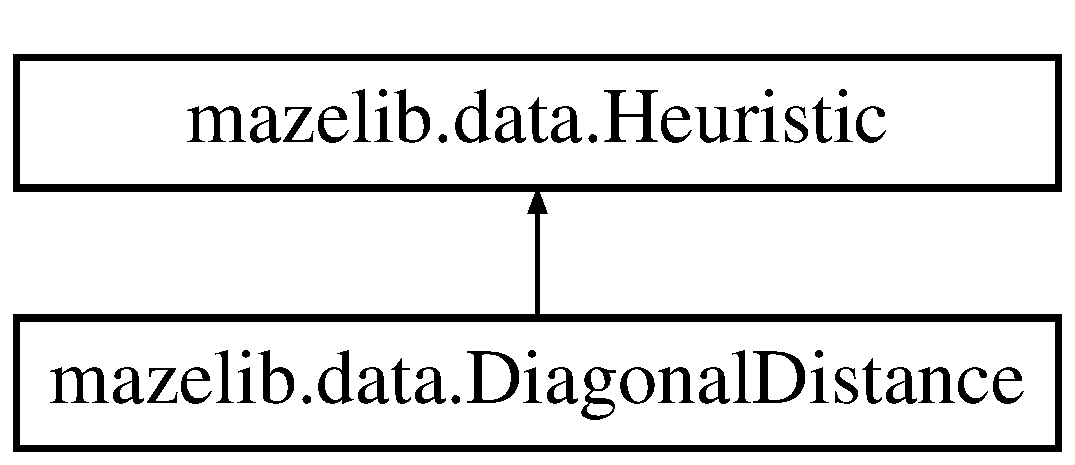
\includegraphics[height=2.000000cm]{classmazelib_1_1data_1_1_diagonal_distance}
\end{center}
\end{figure}
\subsection*{Public Member Functions}
\begin{DoxyCompactItemize}
\item 
\hypertarget{classmazelib_1_1data_1_1_diagonal_distance_a5d0d1ab0b905edd45bbec8f4ad82f371}{long {\bfseries calculate\-Distance} (\hyperlink{classmazelib_1_1data_1_1_node}{Node} origin\-Node, \hyperlink{classmazelib_1_1data_1_1_node}{Node} target\-Node)}\label{classmazelib_1_1data_1_1_diagonal_distance_a5d0d1ab0b905edd45bbec8f4ad82f371}

\end{DoxyCompactItemize}


\subsection{Detailed Description}
\hyperlink{classmazelib_1_1data_1_1_maze}{Maze} Algorithm \hyperlink{interfacemazelib_1_1data_1_1_heuristic}{Heuristic} to calculate Diagonal Distance. \begin{DoxyAuthor}{Author}
Timur Reziapov \href{mailto:reziapo1@illinois.edu}{\tt reziapo1@illinois.\-edu} 
\end{DoxyAuthor}
\begin{DoxyDate}{Date}
Sunday, September 9, 2012 18\-:00 P\-M 
\end{DoxyDate}


The documentation for this class was generated from the following file\-:\begin{DoxyCompactItemize}
\item 
src/mazelib/data/Diagonal\-Distance.\-java\end{DoxyCompactItemize}

\hypertarget{classmazelib_1_1data_1_1_dijkstras_algorithm}{\section{mazelib.\-data.\-Dijkstras\-Algorithm Class Reference}
\label{classmazelib_1_1data_1_1_dijkstras_algorithm}\index{mazelib.\-data.\-Dijkstras\-Algorithm@{mazelib.\-data.\-Dijkstras\-Algorithm}}
}
Inheritance diagram for mazelib.\-data.\-Dijkstras\-Algorithm\-:\begin{figure}[H]
\begin{center}
\leavevmode
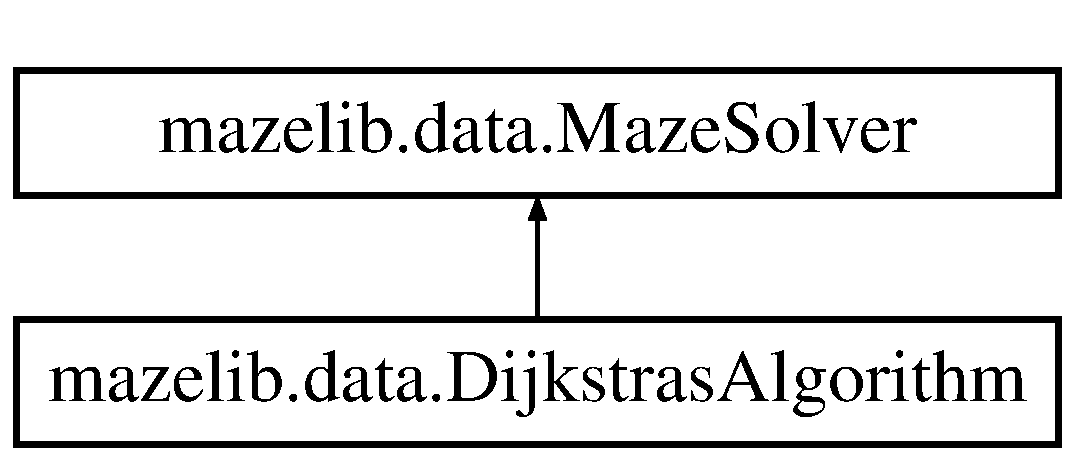
\includegraphics[height=2.000000cm]{classmazelib_1_1data_1_1_dijkstras_algorithm}
\end{center}
\end{figure}
\subsection*{Public Member Functions}
\begin{DoxyCompactItemize}
\item 
\hyperlink{classmazelib_1_1data_1_1_dijkstras_algorithm_ade11d276ab1b7c542eb6860c483924d2}{Dijkstras\-Algorithm} (\hyperlink{classmazelib_1_1data_1_1_maze}{Maze} maze, \hyperlink{interfacemazelib_1_1data_1_1_heuristic}{Heuristic} heuristic)
\item 
\hyperlink{classmazelib_1_1data_1_1_dijkstras_algorithm_ad956882a012e15144eb3339746105497}{Dijkstras\-Algorithm} (String string\-Maze, \hyperlink{interfacemazelib_1_1data_1_1_heuristic}{Heuristic} heuristic)
\item 
List$<$ \hyperlink{classmazelib_1_1data_1_1_node}{Node} $>$ \hyperlink{classmazelib_1_1data_1_1_dijkstras_algorithm_abe1208942d2a0397235aef4737990ca2}{solve\-Maze} ()
\end{DoxyCompactItemize}
\subsection*{Additional Inherited Members}


\subsection{Detailed Description}
\begin{DoxyAuthor}{Author}
Timur Reziapov \href{mailto:reziapo1@illinois.edu}{\tt reziapo1@illinois.\-edu} 
\end{DoxyAuthor}
\begin{DoxyDate}{Date}
Sunday, September 9, 2012 18\-:00 P\-M 
\end{DoxyDate}


\subsection{Constructor \& Destructor Documentation}
\hypertarget{classmazelib_1_1data_1_1_dijkstras_algorithm_ade11d276ab1b7c542eb6860c483924d2}{\index{mazelib\-::data\-::\-Dijkstras\-Algorithm@{mazelib\-::data\-::\-Dijkstras\-Algorithm}!Dijkstras\-Algorithm@{Dijkstras\-Algorithm}}
\index{Dijkstras\-Algorithm@{Dijkstras\-Algorithm}!mazelib::data::DijkstrasAlgorithm@{mazelib\-::data\-::\-Dijkstras\-Algorithm}}
\subsubsection[{Dijkstras\-Algorithm}]{\setlength{\rightskip}{0pt plus 5cm}mazelib.\-data.\-Dijkstras\-Algorithm.\-Dijkstras\-Algorithm (
\begin{DoxyParamCaption}
\item[{{\bf Maze}}]{maze, }
\item[{{\bf Heuristic}}]{heuristic}
\end{DoxyParamCaption}
)\hspace{0.3cm}{\ttfamily [inline]}}}\label{classmazelib_1_1data_1_1_dijkstras_algorithm_ade11d276ab1b7c542eb6860c483924d2}
Constructor for Dijkastras\-Algorithm Object. 
\begin{DoxyParams}{Parameters}
{\em maze} & the \hyperlink{classmazelib_1_1data_1_1_maze}{Maze} to solve \\
\hline
\end{DoxyParams}
\hypertarget{classmazelib_1_1data_1_1_dijkstras_algorithm_ad956882a012e15144eb3339746105497}{\index{mazelib\-::data\-::\-Dijkstras\-Algorithm@{mazelib\-::data\-::\-Dijkstras\-Algorithm}!Dijkstras\-Algorithm@{Dijkstras\-Algorithm}}
\index{Dijkstras\-Algorithm@{Dijkstras\-Algorithm}!mazelib::data::DijkstrasAlgorithm@{mazelib\-::data\-::\-Dijkstras\-Algorithm}}
\subsubsection[{Dijkstras\-Algorithm}]{\setlength{\rightskip}{0pt plus 5cm}mazelib.\-data.\-Dijkstras\-Algorithm.\-Dijkstras\-Algorithm (
\begin{DoxyParamCaption}
\item[{String}]{string\-Maze, }
\item[{{\bf Heuristic}}]{heuristic}
\end{DoxyParamCaption}
)\hspace{0.3cm}{\ttfamily [inline]}}}\label{classmazelib_1_1data_1_1_dijkstras_algorithm_ad956882a012e15144eb3339746105497}
Constructor for \hyperlink{classmazelib_1_1data_1_1_dijkstras_algorithm}{Dijkstras\-Algorithm} Object. 
\begin{DoxyParams}{Parameters}
{\em string\-Maze} & the string representation of the \hyperlink{classmazelib_1_1data_1_1_maze}{Maze} to solve \\
\hline
\end{DoxyParams}


\subsection{Member Function Documentation}
\hypertarget{classmazelib_1_1data_1_1_dijkstras_algorithm_abe1208942d2a0397235aef4737990ca2}{\index{mazelib\-::data\-::\-Dijkstras\-Algorithm@{mazelib\-::data\-::\-Dijkstras\-Algorithm}!solve\-Maze@{solve\-Maze}}
\index{solve\-Maze@{solve\-Maze}!mazelib::data::DijkstrasAlgorithm@{mazelib\-::data\-::\-Dijkstras\-Algorithm}}
\subsubsection[{solve\-Maze}]{\setlength{\rightskip}{0pt plus 5cm}List$<${\bf Node}$>$ mazelib.\-data.\-Dijkstras\-Algorithm.\-solve\-Maze (
\begin{DoxyParamCaption}
{}
\end{DoxyParamCaption}
)\hspace{0.3cm}{\ttfamily [inline]}, {\ttfamily [virtual]}}}\label{classmazelib_1_1data_1_1_dijkstras_algorithm_abe1208942d2a0397235aef4737990ca2}
The main function of the algorithm. 

Implements \hyperlink{classmazelib_1_1data_1_1_maze_solver_a009bd983cdccfb7c845d3da8fabf02d6}{mazelib.\-data.\-Maze\-Solver}.



The documentation for this class was generated from the following file\-:\begin{DoxyCompactItemize}
\item 
src/mazelib/data/Dijkstras\-Algorithm.\-java\end{DoxyCompactItemize}

\hypertarget{classmazelib_1_1tests_1_1_dijkstras_algorithm_test}{\section{mazelib.\-tests.\-Dijkstras\-Algorithm\-Test Class Reference}
\label{classmazelib_1_1tests_1_1_dijkstras_algorithm_test}\index{mazelib.\-tests.\-Dijkstras\-Algorithm\-Test@{mazelib.\-tests.\-Dijkstras\-Algorithm\-Test}}
}
\subsection*{Public Member Functions}
\begin{DoxyCompactItemize}
\item 
void \hyperlink{classmazelib_1_1tests_1_1_dijkstras_algorithm_test_a1146e87fe1b5efcbbaa60fe88ab1ce08}{test\-Initialization} ()
\item 
void \hyperlink{classmazelib_1_1tests_1_1_dijkstras_algorithm_test_a2d20a1359ec9953b68e5c80d6b74e7fe}{test\-Main\-Exceptions} ()
\item 
void \hyperlink{classmazelib_1_1tests_1_1_dijkstras_algorithm_test_a89d3538fea9ac9435d3c10969c457c26}{test\-Open\-Area} ()
\item 
void \hyperlink{classmazelib_1_1tests_1_1_dijkstras_algorithm_test_a8a89aea0f3368802dfa118d8c7b38d72}{test\-Wall} ()
\item 
void \hyperlink{classmazelib_1_1tests_1_1_dijkstras_algorithm_test_abb427a3019f7e4886d718c9f026b57f7}{test\-Wall\-Bottom} ()
\item 
void \hyperlink{classmazelib_1_1tests_1_1_dijkstras_algorithm_test_afeec52b72833744e39ba281094dd96ec}{test\-Choose\-Shortest\-Path} ()
\item 
void \hyperlink{classmazelib_1_1tests_1_1_dijkstras_algorithm_test_a5bdb0931d622a52508b992fb9830efe8}{test\-Big\-Maze} ()
\item 
void \hyperlink{classmazelib_1_1tests_1_1_dijkstras_algorithm_test_a5a2da8268b9e90f3147d7a3275a69ad9}{test\-Unsolvable} ()
\item 
void \hyperlink{classmazelib_1_1tests_1_1_dijkstras_algorithm_test_a44771de70f3330345536faaf5e7d3d0d}{test\-Unsolvable\-Diagonal} ()
\item 
void \hyperlink{classmazelib_1_1tests_1_1_dijkstras_algorithm_test_af7b54eea5de705c27e280eefe3c83cd5}{test\-Heuristic\-Independence} ()
\item 
void \hyperlink{classmazelib_1_1tests_1_1_dijkstras_algorithm_test_a509f7c865dbe035833a3afd30585f9b2}{test\-Draw\-Solution} ()
\end{DoxyCompactItemize}


\subsection{Detailed Description}
\begin{DoxyAuthor}{Author}
Timur Reziapov \href{mailto:reziapo1@illinois.edu}{\tt reziapo1@illinois.\-edu} 
\end{DoxyAuthor}
\begin{DoxyDate}{Date}
Tuesday, September 11, 2012, 18\-:00 P\-M 
\end{DoxyDate}


\subsection{Member Function Documentation}
\hypertarget{classmazelib_1_1tests_1_1_dijkstras_algorithm_test_a5bdb0931d622a52508b992fb9830efe8}{\index{mazelib\-::tests\-::\-Dijkstras\-Algorithm\-Test@{mazelib\-::tests\-::\-Dijkstras\-Algorithm\-Test}!test\-Big\-Maze@{test\-Big\-Maze}}
\index{test\-Big\-Maze@{test\-Big\-Maze}!mazelib::tests::DijkstrasAlgorithmTest@{mazelib\-::tests\-::\-Dijkstras\-Algorithm\-Test}}
\subsubsection[{test\-Big\-Maze}]{\setlength{\rightskip}{0pt plus 5cm}void mazelib.\-tests.\-Dijkstras\-Algorithm\-Test.\-test\-Big\-Maze (
\begin{DoxyParamCaption}
{}
\end{DoxyParamCaption}
)\hspace{0.3cm}{\ttfamily [inline]}}}\label{classmazelib_1_1tests_1_1_dijkstras_algorithm_test_a5bdb0931d622a52508b992fb9830efe8}
This test checks if the algorithm can solve relatively big Mazes. \hypertarget{classmazelib_1_1tests_1_1_dijkstras_algorithm_test_afeec52b72833744e39ba281094dd96ec}{\index{mazelib\-::tests\-::\-Dijkstras\-Algorithm\-Test@{mazelib\-::tests\-::\-Dijkstras\-Algorithm\-Test}!test\-Choose\-Shortest\-Path@{test\-Choose\-Shortest\-Path}}
\index{test\-Choose\-Shortest\-Path@{test\-Choose\-Shortest\-Path}!mazelib::tests::DijkstrasAlgorithmTest@{mazelib\-::tests\-::\-Dijkstras\-Algorithm\-Test}}
\subsubsection[{test\-Choose\-Shortest\-Path}]{\setlength{\rightskip}{0pt plus 5cm}void mazelib.\-tests.\-Dijkstras\-Algorithm\-Test.\-test\-Choose\-Shortest\-Path (
\begin{DoxyParamCaption}
{}
\end{DoxyParamCaption}
)\hspace{0.3cm}{\ttfamily [inline]}}}\label{classmazelib_1_1tests_1_1_dijkstras_algorithm_test_afeec52b72833744e39ba281094dd96ec}
This test checks if solver chooses the shortest path when there are multiple paths leading to the end Node. Shortest path is the one with most diagonal moves. \hypertarget{classmazelib_1_1tests_1_1_dijkstras_algorithm_test_a509f7c865dbe035833a3afd30585f9b2}{\index{mazelib\-::tests\-::\-Dijkstras\-Algorithm\-Test@{mazelib\-::tests\-::\-Dijkstras\-Algorithm\-Test}!test\-Draw\-Solution@{test\-Draw\-Solution}}
\index{test\-Draw\-Solution@{test\-Draw\-Solution}!mazelib::tests::DijkstrasAlgorithmTest@{mazelib\-::tests\-::\-Dijkstras\-Algorithm\-Test}}
\subsubsection[{test\-Draw\-Solution}]{\setlength{\rightskip}{0pt plus 5cm}void mazelib.\-tests.\-Dijkstras\-Algorithm\-Test.\-test\-Draw\-Solution (
\begin{DoxyParamCaption}
{}
\end{DoxyParamCaption}
)\hspace{0.3cm}{\ttfamily [inline]}}}\label{classmazelib_1_1tests_1_1_dijkstras_algorithm_test_a509f7c865dbe035833a3afd30585f9b2}
This test checks if draw\-Solutiion returns the same output if called twice and returns a String representation of successfully solved maze. \hypertarget{classmazelib_1_1tests_1_1_dijkstras_algorithm_test_af7b54eea5de705c27e280eefe3c83cd5}{\index{mazelib\-::tests\-::\-Dijkstras\-Algorithm\-Test@{mazelib\-::tests\-::\-Dijkstras\-Algorithm\-Test}!test\-Heuristic\-Independence@{test\-Heuristic\-Independence}}
\index{test\-Heuristic\-Independence@{test\-Heuristic\-Independence}!mazelib::tests::DijkstrasAlgorithmTest@{mazelib\-::tests\-::\-Dijkstras\-Algorithm\-Test}}
\subsubsection[{test\-Heuristic\-Independence}]{\setlength{\rightskip}{0pt plus 5cm}void mazelib.\-tests.\-Dijkstras\-Algorithm\-Test.\-test\-Heuristic\-Independence (
\begin{DoxyParamCaption}
{}
\end{DoxyParamCaption}
)\hspace{0.3cm}{\ttfamily [inline]}}}\label{classmazelib_1_1tests_1_1_dijkstras_algorithm_test_af7b54eea5de705c27e280eefe3c83cd5}
This test checks if Mazes are solveable regardless of the Heuristic used. \hypertarget{classmazelib_1_1tests_1_1_dijkstras_algorithm_test_a1146e87fe1b5efcbbaa60fe88ab1ce08}{\index{mazelib\-::tests\-::\-Dijkstras\-Algorithm\-Test@{mazelib\-::tests\-::\-Dijkstras\-Algorithm\-Test}!test\-Initialization@{test\-Initialization}}
\index{test\-Initialization@{test\-Initialization}!mazelib::tests::DijkstrasAlgorithmTest@{mazelib\-::tests\-::\-Dijkstras\-Algorithm\-Test}}
\subsubsection[{test\-Initialization}]{\setlength{\rightskip}{0pt plus 5cm}void mazelib.\-tests.\-Dijkstras\-Algorithm\-Test.\-test\-Initialization (
\begin{DoxyParamCaption}
{}
\end{DoxyParamCaption}
)\hspace{0.3cm}{\ttfamily [inline]}}}\label{classmazelib_1_1tests_1_1_dijkstras_algorithm_test_a1146e87fe1b5efcbbaa60fe88ab1ce08}
Test to check A\-Start\-Algorithm object initialization. Checks both Maze and String constructors. \hypertarget{classmazelib_1_1tests_1_1_dijkstras_algorithm_test_a2d20a1359ec9953b68e5c80d6b74e7fe}{\index{mazelib\-::tests\-::\-Dijkstras\-Algorithm\-Test@{mazelib\-::tests\-::\-Dijkstras\-Algorithm\-Test}!test\-Main\-Exceptions@{test\-Main\-Exceptions}}
\index{test\-Main\-Exceptions@{test\-Main\-Exceptions}!mazelib::tests::DijkstrasAlgorithmTest@{mazelib\-::tests\-::\-Dijkstras\-Algorithm\-Test}}
\subsubsection[{test\-Main\-Exceptions}]{\setlength{\rightskip}{0pt plus 5cm}void mazelib.\-tests.\-Dijkstras\-Algorithm\-Test.\-test\-Main\-Exceptions (
\begin{DoxyParamCaption}
{}
\end{DoxyParamCaption}
)\hspace{0.3cm}{\ttfamily [inline]}}}\label{classmazelib_1_1tests_1_1_dijkstras_algorithm_test_a2d20a1359ec9953b68e5c80d6b74e7fe}
Test to check if main function causes any exceptions. \hypertarget{classmazelib_1_1tests_1_1_dijkstras_algorithm_test_a89d3538fea9ac9435d3c10969c457c26}{\index{mazelib\-::tests\-::\-Dijkstras\-Algorithm\-Test@{mazelib\-::tests\-::\-Dijkstras\-Algorithm\-Test}!test\-Open\-Area@{test\-Open\-Area}}
\index{test\-Open\-Area@{test\-Open\-Area}!mazelib::tests::DijkstrasAlgorithmTest@{mazelib\-::tests\-::\-Dijkstras\-Algorithm\-Test}}
\subsubsection[{test\-Open\-Area}]{\setlength{\rightskip}{0pt plus 5cm}void mazelib.\-tests.\-Dijkstras\-Algorithm\-Test.\-test\-Open\-Area (
\begin{DoxyParamCaption}
{}
\end{DoxyParamCaption}
)\hspace{0.3cm}{\ttfamily [inline]}}}\label{classmazelib_1_1tests_1_1_dijkstras_algorithm_test_a89d3538fea9ac9435d3c10969c457c26}
This test checks if the algorithm can find a way in an area with no walls. \hypertarget{classmazelib_1_1tests_1_1_dijkstras_algorithm_test_a5a2da8268b9e90f3147d7a3275a69ad9}{\index{mazelib\-::tests\-::\-Dijkstras\-Algorithm\-Test@{mazelib\-::tests\-::\-Dijkstras\-Algorithm\-Test}!test\-Unsolvable@{test\-Unsolvable}}
\index{test\-Unsolvable@{test\-Unsolvable}!mazelib::tests::DijkstrasAlgorithmTest@{mazelib\-::tests\-::\-Dijkstras\-Algorithm\-Test}}
\subsubsection[{test\-Unsolvable}]{\setlength{\rightskip}{0pt plus 5cm}void mazelib.\-tests.\-Dijkstras\-Algorithm\-Test.\-test\-Unsolvable (
\begin{DoxyParamCaption}
{}
\end{DoxyParamCaption}
)\hspace{0.3cm}{\ttfamily [inline]}}}\label{classmazelib_1_1tests_1_1_dijkstras_algorithm_test_a5a2da8268b9e90f3147d7a3275a69ad9}
This test checks if the algorithm handles mazes where target is blocked by walls. \hypertarget{classmazelib_1_1tests_1_1_dijkstras_algorithm_test_a44771de70f3330345536faaf5e7d3d0d}{\index{mazelib\-::tests\-::\-Dijkstras\-Algorithm\-Test@{mazelib\-::tests\-::\-Dijkstras\-Algorithm\-Test}!test\-Unsolvable\-Diagonal@{test\-Unsolvable\-Diagonal}}
\index{test\-Unsolvable\-Diagonal@{test\-Unsolvable\-Diagonal}!mazelib::tests::DijkstrasAlgorithmTest@{mazelib\-::tests\-::\-Dijkstras\-Algorithm\-Test}}
\subsubsection[{test\-Unsolvable\-Diagonal}]{\setlength{\rightskip}{0pt plus 5cm}void mazelib.\-tests.\-Dijkstras\-Algorithm\-Test.\-test\-Unsolvable\-Diagonal (
\begin{DoxyParamCaption}
{}
\end{DoxyParamCaption}
)\hspace{0.3cm}{\ttfamily [inline]}}}\label{classmazelib_1_1tests_1_1_dijkstras_algorithm_test_a44771de70f3330345536faaf5e7d3d0d}
This test checks if the algorithm handles mazes where target isn't surrounded by walls but can't be reached diagonally. \hypertarget{classmazelib_1_1tests_1_1_dijkstras_algorithm_test_a8a89aea0f3368802dfa118d8c7b38d72}{\index{mazelib\-::tests\-::\-Dijkstras\-Algorithm\-Test@{mazelib\-::tests\-::\-Dijkstras\-Algorithm\-Test}!test\-Wall@{test\-Wall}}
\index{test\-Wall@{test\-Wall}!mazelib::tests::DijkstrasAlgorithmTest@{mazelib\-::tests\-::\-Dijkstras\-Algorithm\-Test}}
\subsubsection[{test\-Wall}]{\setlength{\rightskip}{0pt plus 5cm}void mazelib.\-tests.\-Dijkstras\-Algorithm\-Test.\-test\-Wall (
\begin{DoxyParamCaption}
{}
\end{DoxyParamCaption}
)\hspace{0.3cm}{\ttfamily [inline]}}}\label{classmazelib_1_1tests_1_1_dijkstras_algorithm_test_a8a89aea0f3368802dfa118d8c7b38d72}
This test checks if the algorithm can find a way blocked by a wall. \hypertarget{classmazelib_1_1tests_1_1_dijkstras_algorithm_test_abb427a3019f7e4886d718c9f026b57f7}{\index{mazelib\-::tests\-::\-Dijkstras\-Algorithm\-Test@{mazelib\-::tests\-::\-Dijkstras\-Algorithm\-Test}!test\-Wall\-Bottom@{test\-Wall\-Bottom}}
\index{test\-Wall\-Bottom@{test\-Wall\-Bottom}!mazelib::tests::DijkstrasAlgorithmTest@{mazelib\-::tests\-::\-Dijkstras\-Algorithm\-Test}}
\subsubsection[{test\-Wall\-Bottom}]{\setlength{\rightskip}{0pt plus 5cm}void mazelib.\-tests.\-Dijkstras\-Algorithm\-Test.\-test\-Wall\-Bottom (
\begin{DoxyParamCaption}
{}
\end{DoxyParamCaption}
)\hspace{0.3cm}{\ttfamily [inline]}}}\label{classmazelib_1_1tests_1_1_dijkstras_algorithm_test_abb427a3019f7e4886d718c9f026b57f7}
This test checks if the algorithm can find a way blocked by a wall at the bottom 

The documentation for this class was generated from the following file\-:\begin{DoxyCompactItemize}
\item 
src/mazelib/tests/Dijkstras\-Algorithm\-Test.\-java\end{DoxyCompactItemize}

\hypertarget{classmazelib_1_1data_1_1_euclidean_distance}{\section{mazelib.\-data.\-Euclidean\-Distance Class Reference}
\label{classmazelib_1_1data_1_1_euclidean_distance}\index{mazelib.\-data.\-Euclidean\-Distance@{mazelib.\-data.\-Euclidean\-Distance}}
}
Inheritance diagram for mazelib.\-data.\-Euclidean\-Distance\-:\begin{figure}[H]
\begin{center}
\leavevmode
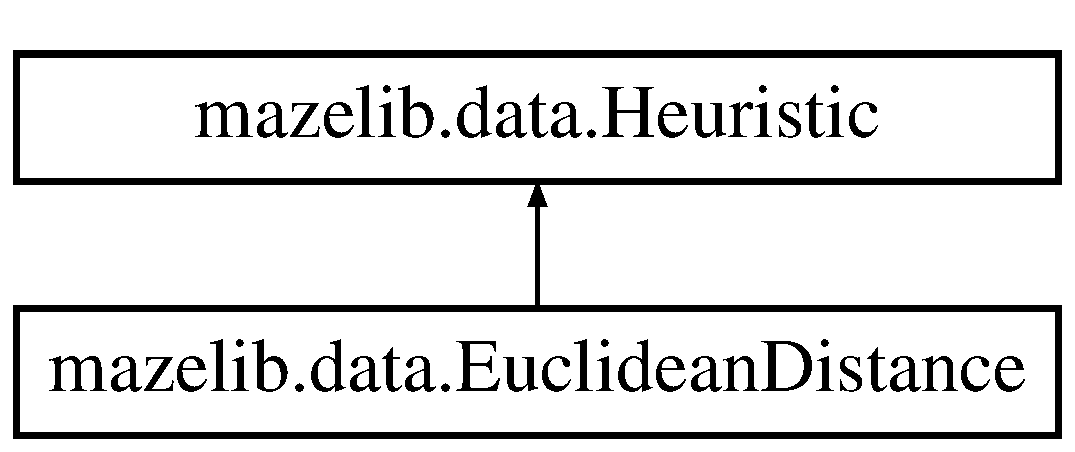
\includegraphics[height=2.000000cm]{classmazelib_1_1data_1_1_euclidean_distance}
\end{center}
\end{figure}
\subsection*{Public Member Functions}
\begin{DoxyCompactItemize}
\item 
long \hyperlink{classmazelib_1_1data_1_1_euclidean_distance_ad25a60eeb1a8bbe3d7c428d125e02320}{calculate\-Distance} (\hyperlink{classmazelib_1_1data_1_1_node}{Node} origin\-Node, \hyperlink{classmazelib_1_1data_1_1_node}{Node} target\-Node)
\end{DoxyCompactItemize}


\subsection{Detailed Description}
\hyperlink{classmazelib_1_1data_1_1_maze}{Maze} Algorithm \hyperlink{interfacemazelib_1_1data_1_1_heuristic}{Heuristic} to calculate Euclidean Distance. \begin{DoxyAuthor}{Author}
Timur Reziapov \href{mailto:reziapo1@illinois.edu}{\tt reziapo1@illinois.\-edu} 
\end{DoxyAuthor}
\begin{DoxyDate}{Date}
Sunday, September 9, 2012 18\-:00 P\-M 
\end{DoxyDate}


\subsection{Member Function Documentation}
\hypertarget{classmazelib_1_1data_1_1_euclidean_distance_ad25a60eeb1a8bbe3d7c428d125e02320}{\index{mazelib\-::data\-::\-Euclidean\-Distance@{mazelib\-::data\-::\-Euclidean\-Distance}!calculate\-Distance@{calculate\-Distance}}
\index{calculate\-Distance@{calculate\-Distance}!mazelib::data::EuclideanDistance@{mazelib\-::data\-::\-Euclidean\-Distance}}
\subsubsection[{calculate\-Distance}]{\setlength{\rightskip}{0pt plus 5cm}long mazelib.\-data.\-Euclidean\-Distance.\-calculate\-Distance (
\begin{DoxyParamCaption}
\item[{{\bf Node}}]{origin\-Node, }
\item[{{\bf Node}}]{target\-Node}
\end{DoxyParamCaption}
)\hspace{0.3cm}{\ttfamily [inline]}}}\label{classmazelib_1_1data_1_1_euclidean_distance_ad25a60eeb1a8bbe3d7c428d125e02320}
Calculate distance in straight direction to target 
\begin{DoxyParams}{Parameters}
{\em origin\-Node} & the \hyperlink{classmazelib_1_1data_1_1_node}{Node} to calculate distance from \\
\hline
{\em target\-Node} & the \hyperlink{classmazelib_1_1data_1_1_node}{Node} to calculate distance to \\
\hline
\end{DoxyParams}
\begin{DoxyReturn}{Returns}
the Distance from origin to end in a straight line 
\end{DoxyReturn}


The documentation for this class was generated from the following file\-:\begin{DoxyCompactItemize}
\item 
src/mazelib/data/Euclidean\-Distance.\-java\end{DoxyCompactItemize}

\hypertarget{interfacemazelib_1_1data_1_1_heuristic}{\section{mazelib.\-data.\-Heuristic Interface Reference}
\label{interfacemazelib_1_1data_1_1_heuristic}\index{mazelib.\-data.\-Heuristic@{mazelib.\-data.\-Heuristic}}
}
Inheritance diagram for mazelib.\-data.\-Heuristic\-:\begin{figure}[H]
\begin{center}
\leavevmode
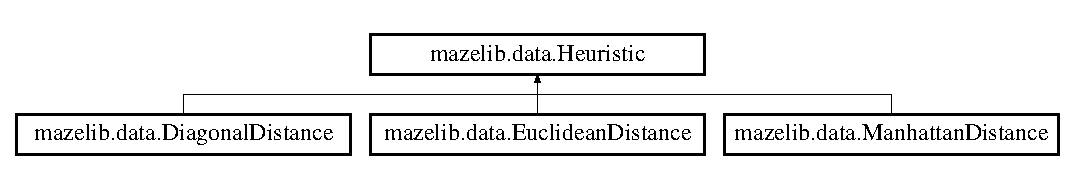
\includegraphics[height=1.848185cm]{interfacemazelib_1_1data_1_1_heuristic}
\end{center}
\end{figure}
\subsection*{Public Member Functions}
\begin{DoxyCompactItemize}
\item 
long \hyperlink{interfacemazelib_1_1data_1_1_heuristic_a740b90bd253ed4ef33c7f18f8011215f}{calculate\-Distance} (\hyperlink{classmazelib_1_1data_1_1_node}{Node} origin\-Node, \hyperlink{classmazelib_1_1data_1_1_node}{Node} target\-Node)
\end{DoxyCompactItemize}


\subsection{Detailed Description}
Interface to facilitate pluggable Algorithm Heuristics. \begin{DoxyAuthor}{Author}
Timur Reziapov \href{mailto:reziapo1@illinois.edu}{\tt reziapo1@illinois.\-edu} 
\end{DoxyAuthor}
\begin{DoxyDate}{Date}
Sunday, September 9, 2012 18\-:00 P\-M 
\end{DoxyDate}


\subsection{Member Function Documentation}
\hypertarget{interfacemazelib_1_1data_1_1_heuristic_a740b90bd253ed4ef33c7f18f8011215f}{\index{mazelib\-::data\-::\-Heuristic@{mazelib\-::data\-::\-Heuristic}!calculate\-Distance@{calculate\-Distance}}
\index{calculate\-Distance@{calculate\-Distance}!mazelib::data::Heuristic@{mazelib\-::data\-::\-Heuristic}}
\subsubsection[{calculate\-Distance}]{\setlength{\rightskip}{0pt plus 5cm}long mazelib.\-data.\-Heuristic.\-calculate\-Distance (
\begin{DoxyParamCaption}
\item[{{\bf Node}}]{origin\-Node, }
\item[{{\bf Node}}]{target\-Node}
\end{DoxyParamCaption}
)}}\label{interfacemazelib_1_1data_1_1_heuristic_a740b90bd253ed4ef33c7f18f8011215f}
Method that all implementing classes must define. 
\begin{DoxyParams}{Parameters}
{\em origin\-Node} & the \hyperlink{classmazelib_1_1data_1_1_node}{Node} to calculate distance from \\
\hline
{\em target\-Node} & the \hyperlink{classmazelib_1_1data_1_1_node}{Node} to calculate distance to \\
\hline
\end{DoxyParams}
\begin{DoxyReturn}{Returns}
the distance from origin to target according to the \hyperlink{interfacemazelib_1_1data_1_1_heuristic}{Heuristic} 
\end{DoxyReturn}


The documentation for this interface was generated from the following file\-:\begin{DoxyCompactItemize}
\item 
src/mazelib/data/Heuristic.\-java\end{DoxyCompactItemize}

\hypertarget{classmazelib_1_1tests_1_1_heuristics_test}{\section{mazelib.\-tests.\-Heuristics\-Test Class Reference}
\label{classmazelib_1_1tests_1_1_heuristics_test}\index{mazelib.\-tests.\-Heuristics\-Test@{mazelib.\-tests.\-Heuristics\-Test}}
}
\subsection*{Public Member Functions}
\begin{DoxyCompactItemize}
\item 
void \hyperlink{classmazelib_1_1tests_1_1_heuristics_test_a825dc5d9bf79db08ad843080b0e72b7b}{test\-Manhattan\-Distance} ()
\item 
void \hyperlink{classmazelib_1_1tests_1_1_heuristics_test_a4a027f794b8e182bf3ae5703e8dd103f}{test\-Euclidean\-Distance} ()
\item 
void \hyperlink{classmazelib_1_1tests_1_1_heuristics_test_ab6264fc89c89e6d0aec1985c0b4cb95d}{test\-Diagonal\-Distance} ()
\end{DoxyCompactItemize}
\subsection*{Static Public Member Functions}
\begin{DoxyCompactItemize}
\item 
static void \hyperlink{classmazelib_1_1tests_1_1_heuristics_test_a3854f2461cbcbad011be38c4c47b0350}{set\-Up\-Before\-Class} ()  throws Exception 
\end{DoxyCompactItemize}


\subsection{Detailed Description}
\begin{DoxyAuthor}{Author}
Timur Reziapov \href{mailto:reziapo1@illinois.edu}{\tt reziapo1@illinois.\-edu} 
\end{DoxyAuthor}
\begin{DoxyDate}{Date}
Tuesday, September 11, 2012, 18\-:00 P\-M 
\end{DoxyDate}


\subsection{Member Function Documentation}
\hypertarget{classmazelib_1_1tests_1_1_heuristics_test_a3854f2461cbcbad011be38c4c47b0350}{\index{mazelib\-::tests\-::\-Heuristics\-Test@{mazelib\-::tests\-::\-Heuristics\-Test}!set\-Up\-Before\-Class@{set\-Up\-Before\-Class}}
\index{set\-Up\-Before\-Class@{set\-Up\-Before\-Class}!mazelib::tests::HeuristicsTest@{mazelib\-::tests\-::\-Heuristics\-Test}}
\subsubsection[{set\-Up\-Before\-Class}]{\setlength{\rightskip}{0pt plus 5cm}static void mazelib.\-tests.\-Heuristics\-Test.\-set\-Up\-Before\-Class (
\begin{DoxyParamCaption}
{}
\end{DoxyParamCaption}
)  throws Exception \hspace{0.3cm}{\ttfamily [inline]}, {\ttfamily [static]}}}\label{classmazelib_1_1tests_1_1_heuristics_test_a3854f2461cbcbad011be38c4c47b0350}
This test is run before any other tests. 
\begin{DoxyExceptions}{Exceptions}
{\em Exception} & \\
\hline
\end{DoxyExceptions}
\hypertarget{classmazelib_1_1tests_1_1_heuristics_test_ab6264fc89c89e6d0aec1985c0b4cb95d}{\index{mazelib\-::tests\-::\-Heuristics\-Test@{mazelib\-::tests\-::\-Heuristics\-Test}!test\-Diagonal\-Distance@{test\-Diagonal\-Distance}}
\index{test\-Diagonal\-Distance@{test\-Diagonal\-Distance}!mazelib::tests::HeuristicsTest@{mazelib\-::tests\-::\-Heuristics\-Test}}
\subsubsection[{test\-Diagonal\-Distance}]{\setlength{\rightskip}{0pt plus 5cm}void mazelib.\-tests.\-Heuristics\-Test.\-test\-Diagonal\-Distance (
\begin{DoxyParamCaption}
{}
\end{DoxyParamCaption}
)\hspace{0.3cm}{\ttfamily [inline]}}}\label{classmazelib_1_1tests_1_1_heuristics_test_ab6264fc89c89e6d0aec1985c0b4cb95d}
This test checks the Diagonal Distance Heuristic. \hypertarget{classmazelib_1_1tests_1_1_heuristics_test_a4a027f794b8e182bf3ae5703e8dd103f}{\index{mazelib\-::tests\-::\-Heuristics\-Test@{mazelib\-::tests\-::\-Heuristics\-Test}!test\-Euclidean\-Distance@{test\-Euclidean\-Distance}}
\index{test\-Euclidean\-Distance@{test\-Euclidean\-Distance}!mazelib::tests::HeuristicsTest@{mazelib\-::tests\-::\-Heuristics\-Test}}
\subsubsection[{test\-Euclidean\-Distance}]{\setlength{\rightskip}{0pt plus 5cm}void mazelib.\-tests.\-Heuristics\-Test.\-test\-Euclidean\-Distance (
\begin{DoxyParamCaption}
{}
\end{DoxyParamCaption}
)\hspace{0.3cm}{\ttfamily [inline]}}}\label{classmazelib_1_1tests_1_1_heuristics_test_a4a027f794b8e182bf3ae5703e8dd103f}
This test checks the Euclidean Distance Heuristic. \hypertarget{classmazelib_1_1tests_1_1_heuristics_test_a825dc5d9bf79db08ad843080b0e72b7b}{\index{mazelib\-::tests\-::\-Heuristics\-Test@{mazelib\-::tests\-::\-Heuristics\-Test}!test\-Manhattan\-Distance@{test\-Manhattan\-Distance}}
\index{test\-Manhattan\-Distance@{test\-Manhattan\-Distance}!mazelib::tests::HeuristicsTest@{mazelib\-::tests\-::\-Heuristics\-Test}}
\subsubsection[{test\-Manhattan\-Distance}]{\setlength{\rightskip}{0pt plus 5cm}void mazelib.\-tests.\-Heuristics\-Test.\-test\-Manhattan\-Distance (
\begin{DoxyParamCaption}
{}
\end{DoxyParamCaption}
)\hspace{0.3cm}{\ttfamily [inline]}}}\label{classmazelib_1_1tests_1_1_heuristics_test_a825dc5d9bf79db08ad843080b0e72b7b}
This test checks the Manhattan Distance Heuristic. 

The documentation for this class was generated from the following file\-:\begin{DoxyCompactItemize}
\item 
src/mazelib/tests/Heuristics\-Test.\-java\end{DoxyCompactItemize}

\hypertarget{classmazelib_1_1data_1_1_manhattan_distance}{\section{mazelib.\-data.\-Manhattan\-Distance Class Reference}
\label{classmazelib_1_1data_1_1_manhattan_distance}\index{mazelib.\-data.\-Manhattan\-Distance@{mazelib.\-data.\-Manhattan\-Distance}}
}
Inheritance diagram for mazelib.\-data.\-Manhattan\-Distance\-:\begin{figure}[H]
\begin{center}
\leavevmode
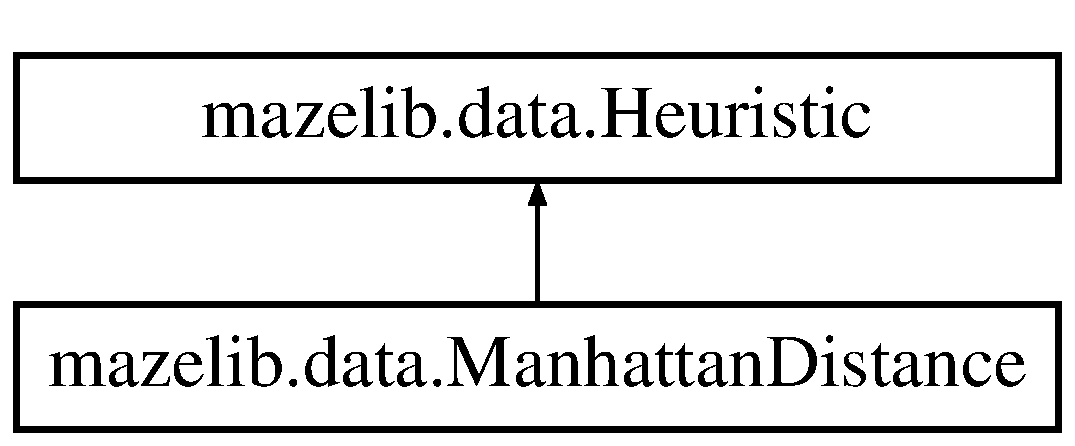
\includegraphics[height=2.000000cm]{classmazelib_1_1data_1_1_manhattan_distance}
\end{center}
\end{figure}
\subsection*{Public Member Functions}
\begin{DoxyCompactItemize}
\item 
long \hyperlink{classmazelib_1_1data_1_1_manhattan_distance_a18e097103b5b7e859b3f5d551ebcffe4}{calculate\-Distance} (\hyperlink{classmazelib_1_1data_1_1_node}{Node} origin\-Node, \hyperlink{classmazelib_1_1data_1_1_node}{Node} target\-Node)
\end{DoxyCompactItemize}


\subsection{Detailed Description}
\hyperlink{classmazelib_1_1data_1_1_maze}{Maze} Algorithm \hyperlink{interfacemazelib_1_1data_1_1_heuristic}{Heuristic} to calculate Manhattan Distance. \begin{DoxyAuthor}{Author}
Timur Reziapov \href{mailto:reziapo1@illinois.edu}{\tt reziapo1@illinois.\-edu} 
\end{DoxyAuthor}
\begin{DoxyDate}{Date}
Sunday, September 9, 2012 18\-:00 P\-M 
\end{DoxyDate}


\subsection{Member Function Documentation}
\hypertarget{classmazelib_1_1data_1_1_manhattan_distance_a18e097103b5b7e859b3f5d551ebcffe4}{\index{mazelib\-::data\-::\-Manhattan\-Distance@{mazelib\-::data\-::\-Manhattan\-Distance}!calculate\-Distance@{calculate\-Distance}}
\index{calculate\-Distance@{calculate\-Distance}!mazelib::data::ManhattanDistance@{mazelib\-::data\-::\-Manhattan\-Distance}}
\subsubsection[{calculate\-Distance}]{\setlength{\rightskip}{0pt plus 5cm}long mazelib.\-data.\-Manhattan\-Distance.\-calculate\-Distance (
\begin{DoxyParamCaption}
\item[{{\bf Node}}]{origin\-Node, }
\item[{{\bf Node}}]{target\-Node}
\end{DoxyParamCaption}
)\hspace{0.3cm}{\ttfamily [inline]}}}\label{classmazelib_1_1data_1_1_manhattan_distance_a18e097103b5b7e859b3f5d551ebcffe4}
Calculate distance in straight directions. 
\begin{DoxyParams}{Parameters}
{\em origin\-Node} & the \hyperlink{classmazelib_1_1data_1_1_node}{Node} to calculate distance from \\
\hline
{\em target\-Node} & the \hyperlink{classmazelib_1_1data_1_1_node}{Node} to calculate distance to \\
\hline
\end{DoxyParams}
\begin{DoxyReturn}{Returns}
the Manhattan distance from origin to target 
\end{DoxyReturn}


The documentation for this class was generated from the following file\-:\begin{DoxyCompactItemize}
\item 
src/mazelib/data/Manhattan\-Distance.\-java\end{DoxyCompactItemize}

\hypertarget{classmazelib_1_1data_1_1_maze}{\section{mazelib.\-data.\-Maze Class Reference}
\label{classmazelib_1_1data_1_1_maze}\index{mazelib.\-data.\-Maze@{mazelib.\-data.\-Maze}}
}
\subsection*{Public Member Functions}
\begin{DoxyCompactItemize}
\item 
\hyperlink{classmazelib_1_1data_1_1_maze_a8fbac7d6a990f2a4dc0f7a6e9548e021}{Maze} (int width, int height)
\item 
\hyperlink{classmazelib_1_1data_1_1_maze_a6108ac1177218d391d9441a14211c338}{Maze} (String maze)
\item 
String \hyperlink{classmazelib_1_1data_1_1_maze_a01357f91230e3ab0f5b5d2bae333775b}{draw\-Maze} ()
\item 
boolean \hyperlink{classmazelib_1_1data_1_1_maze_a5abf2461af90321c99b60d6d7b6baa2e}{in\-Bounds} (\hyperlink{classmazelib_1_1data_1_1_position}{Position} position)
\item 
\hyperlink{classmazelib_1_1data_1_1_node}{Node} \hyperlink{classmazelib_1_1data_1_1_maze_a4f1d235fd8c7bc3f8afab258b511087f}{get\-Node} (\hyperlink{classmazelib_1_1data_1_1_position}{Position} position)
\item 
int \hyperlink{classmazelib_1_1data_1_1_maze_ad6d361bb62158a9613f29108651963d4}{get\-Width} ()
\item 
int \hyperlink{classmazelib_1_1data_1_1_maze_a119104038e76e9793cce077726685e0c}{get\-Height} ()
\item 
\hyperlink{classmazelib_1_1data_1_1_node}{Node} \hyperlink{classmazelib_1_1data_1_1_maze_acb1b8d241380c174d45540d6185c151d}{get\-Start\-Node} ()
\item 
\hyperlink{classmazelib_1_1data_1_1_node}{Node} \hyperlink{classmazelib_1_1data_1_1_maze_a72da72ea9a5d7acfea2d759fa6df83c0}{get\-End\-Node} ()
\end{DoxyCompactItemize}


\subsection{Detailed Description}
\begin{DoxyAuthor}{Author}
Timur Reziapov \href{mailto:reziapo1@illinois.edu}{\tt reziapo1@illinois.\-edu} 
\end{DoxyAuthor}
\begin{DoxyDate}{Date}
Monday, September 3, 2012, 18\-:00 P\-M 
\end{DoxyDate}


\subsection{Constructor \& Destructor Documentation}
\hypertarget{classmazelib_1_1data_1_1_maze_a8fbac7d6a990f2a4dc0f7a6e9548e021}{\index{mazelib\-::data\-::\-Maze@{mazelib\-::data\-::\-Maze}!Maze@{Maze}}
\index{Maze@{Maze}!mazelib::data::Maze@{mazelib\-::data\-::\-Maze}}
\subsubsection[{Maze}]{\setlength{\rightskip}{0pt plus 5cm}mazelib.\-data.\-Maze.\-Maze (
\begin{DoxyParamCaption}
\item[{int}]{width, }
\item[{int}]{height}
\end{DoxyParamCaption}
)\hspace{0.3cm}{\ttfamily [inline]}}}\label{classmazelib_1_1data_1_1_maze_a8fbac7d6a990f2a4dc0f7a6e9548e021}
Constructs a \hyperlink{classmazelib_1_1data_1_1_maze}{Maze} with random squares. \begin{DoxyNote}{Note}
all Nodes are impassable until \hyperlink{classmazelib_1_1data_1_1_maze}{Maze} generation function is called  width and height will at least be 2 
\end{DoxyNote}
\hypertarget{classmazelib_1_1data_1_1_maze_a6108ac1177218d391d9441a14211c338}{\index{mazelib\-::data\-::\-Maze@{mazelib\-::data\-::\-Maze}!Maze@{Maze}}
\index{Maze@{Maze}!mazelib::data::Maze@{mazelib\-::data\-::\-Maze}}
\subsubsection[{Maze}]{\setlength{\rightskip}{0pt plus 5cm}mazelib.\-data.\-Maze.\-Maze (
\begin{DoxyParamCaption}
\item[{String}]{maze}
\end{DoxyParamCaption}
)\hspace{0.3cm}{\ttfamily [inline]}}}\label{classmazelib_1_1data_1_1_maze_a6108ac1177218d391d9441a14211c338}
Constructs a \hyperlink{classmazelib_1_1data_1_1_maze}{Maze} given a string. 
\begin{DoxyParams}{Parameters}
{\em maze} & the String representation of a \hyperlink{classmazelib_1_1data_1_1_maze}{Maze} object, assumed to be in draw\-Maze's format \\
\hline
\end{DoxyParams}


\subsection{Member Function Documentation}
\hypertarget{classmazelib_1_1data_1_1_maze_a01357f91230e3ab0f5b5d2bae333775b}{\index{mazelib\-::data\-::\-Maze@{mazelib\-::data\-::\-Maze}!draw\-Maze@{draw\-Maze}}
\index{draw\-Maze@{draw\-Maze}!mazelib::data::Maze@{mazelib\-::data\-::\-Maze}}
\subsubsection[{draw\-Maze}]{\setlength{\rightskip}{0pt plus 5cm}String mazelib.\-data.\-Maze.\-draw\-Maze (
\begin{DoxyParamCaption}
{}
\end{DoxyParamCaption}
)\hspace{0.3cm}{\ttfamily [inline]}}}\label{classmazelib_1_1data_1_1_maze_a01357f91230e3ab0f5b5d2bae333775b}
This function creates a String representation of this maze. Key\-: \char`\"{}\-X\char`\"{} -\/ impassable/wall \hyperlink{classmazelib_1_1data_1_1_node}{Node} \char`\"{}\#\char`\"{} -\/ \hyperlink{classmazelib_1_1data_1_1_maze}{Maze} border \char`\"{}\-S\char`\"{} -\/ start \hyperlink{classmazelib_1_1data_1_1_node}{Node} \char`\"{}\-E\char`\"{} -\/ end \hyperlink{classmazelib_1_1data_1_1_node}{Node} \char`\"{} \char`\"{} (space) -\/ passable \hyperlink{classmazelib_1_1data_1_1_node}{Node} \begin{DoxyReturn}{Returns}
String representation of this \hyperlink{classmazelib_1_1data_1_1_maze}{Maze} 
\end{DoxyReturn}
\hypertarget{classmazelib_1_1data_1_1_maze_a72da72ea9a5d7acfea2d759fa6df83c0}{\index{mazelib\-::data\-::\-Maze@{mazelib\-::data\-::\-Maze}!get\-End\-Node@{get\-End\-Node}}
\index{get\-End\-Node@{get\-End\-Node}!mazelib::data::Maze@{mazelib\-::data\-::\-Maze}}
\subsubsection[{get\-End\-Node}]{\setlength{\rightskip}{0pt plus 5cm}{\bf Node} mazelib.\-data.\-Maze.\-get\-End\-Node (
\begin{DoxyParamCaption}
{}
\end{DoxyParamCaption}
)\hspace{0.3cm}{\ttfamily [inline]}}}\label{classmazelib_1_1data_1_1_maze_a72da72ea9a5d7acfea2d759fa6df83c0}
\begin{DoxyReturn}{Returns}
the end \hyperlink{classmazelib_1_1data_1_1_node}{Node} for this \hyperlink{classmazelib_1_1data_1_1_maze}{Maze} 
\end{DoxyReturn}
\hypertarget{classmazelib_1_1data_1_1_maze_a119104038e76e9793cce077726685e0c}{\index{mazelib\-::data\-::\-Maze@{mazelib\-::data\-::\-Maze}!get\-Height@{get\-Height}}
\index{get\-Height@{get\-Height}!mazelib::data::Maze@{mazelib\-::data\-::\-Maze}}
\subsubsection[{get\-Height}]{\setlength{\rightskip}{0pt plus 5cm}int mazelib.\-data.\-Maze.\-get\-Height (
\begin{DoxyParamCaption}
{}
\end{DoxyParamCaption}
)\hspace{0.3cm}{\ttfamily [inline]}}}\label{classmazelib_1_1data_1_1_maze_a119104038e76e9793cce077726685e0c}
\begin{DoxyReturn}{Returns}
height of this \hyperlink{classmazelib_1_1data_1_1_maze}{Maze} 
\end{DoxyReturn}
\hypertarget{classmazelib_1_1data_1_1_maze_a4f1d235fd8c7bc3f8afab258b511087f}{\index{mazelib\-::data\-::\-Maze@{mazelib\-::data\-::\-Maze}!get\-Node@{get\-Node}}
\index{get\-Node@{get\-Node}!mazelib::data::Maze@{mazelib\-::data\-::\-Maze}}
\subsubsection[{get\-Node}]{\setlength{\rightskip}{0pt plus 5cm}{\bf Node} mazelib.\-data.\-Maze.\-get\-Node (
\begin{DoxyParamCaption}
\item[{{\bf Position}}]{position}
\end{DoxyParamCaption}
)\hspace{0.3cm}{\ttfamily [inline]}}}\label{classmazelib_1_1data_1_1_maze_a4f1d235fd8c7bc3f8afab258b511087f}

\begin{DoxyParams}{Parameters}
{\em position} & the \hyperlink{classmazelib_1_1data_1_1_position}{Position} of the desired \hyperlink{classmazelib_1_1data_1_1_node}{Node} \\
\hline
\end{DoxyParams}
\begin{DoxyReturn}{Returns}
\hyperlink{classmazelib_1_1data_1_1_node}{Node} at parameter position if in maze bounds, null if out of maze bounds 
\end{DoxyReturn}
\hypertarget{classmazelib_1_1data_1_1_maze_acb1b8d241380c174d45540d6185c151d}{\index{mazelib\-::data\-::\-Maze@{mazelib\-::data\-::\-Maze}!get\-Start\-Node@{get\-Start\-Node}}
\index{get\-Start\-Node@{get\-Start\-Node}!mazelib::data::Maze@{mazelib\-::data\-::\-Maze}}
\subsubsection[{get\-Start\-Node}]{\setlength{\rightskip}{0pt plus 5cm}{\bf Node} mazelib.\-data.\-Maze.\-get\-Start\-Node (
\begin{DoxyParamCaption}
{}
\end{DoxyParamCaption}
)\hspace{0.3cm}{\ttfamily [inline]}}}\label{classmazelib_1_1data_1_1_maze_acb1b8d241380c174d45540d6185c151d}
\begin{DoxyReturn}{Returns}
the starting \hyperlink{classmazelib_1_1data_1_1_node}{Node} for this \hyperlink{classmazelib_1_1data_1_1_maze}{Maze} 
\end{DoxyReturn}
\hypertarget{classmazelib_1_1data_1_1_maze_ad6d361bb62158a9613f29108651963d4}{\index{mazelib\-::data\-::\-Maze@{mazelib\-::data\-::\-Maze}!get\-Width@{get\-Width}}
\index{get\-Width@{get\-Width}!mazelib::data::Maze@{mazelib\-::data\-::\-Maze}}
\subsubsection[{get\-Width}]{\setlength{\rightskip}{0pt plus 5cm}int mazelib.\-data.\-Maze.\-get\-Width (
\begin{DoxyParamCaption}
{}
\end{DoxyParamCaption}
)\hspace{0.3cm}{\ttfamily [inline]}}}\label{classmazelib_1_1data_1_1_maze_ad6d361bb62158a9613f29108651963d4}
\begin{DoxyReturn}{Returns}
width of this \hyperlink{classmazelib_1_1data_1_1_maze}{Maze} 
\end{DoxyReturn}
\hypertarget{classmazelib_1_1data_1_1_maze_a5abf2461af90321c99b60d6d7b6baa2e}{\index{mazelib\-::data\-::\-Maze@{mazelib\-::data\-::\-Maze}!in\-Bounds@{in\-Bounds}}
\index{in\-Bounds@{in\-Bounds}!mazelib::data::Maze@{mazelib\-::data\-::\-Maze}}
\subsubsection[{in\-Bounds}]{\setlength{\rightskip}{0pt plus 5cm}boolean mazelib.\-data.\-Maze.\-in\-Bounds (
\begin{DoxyParamCaption}
\item[{{\bf Position}}]{position}
\end{DoxyParamCaption}
)\hspace{0.3cm}{\ttfamily [inline]}}}\label{classmazelib_1_1data_1_1_maze_a5abf2461af90321c99b60d6d7b6baa2e}
Checks if parameter is in the bounds of this \hyperlink{classmazelib_1_1data_1_1_maze}{Maze}. 
\begin{DoxyParams}{Parameters}
{\em x} & the x coordinate to be checked \\
\hline
{\em y} & the y coordinate to be checked \\
\hline
\end{DoxyParams}
\begin{DoxyReturn}{Returns}
whether x and y are in the bounds of this \hyperlink{classmazelib_1_1data_1_1_node}{Node}'s \hyperlink{classmazelib_1_1data_1_1_maze}{Maze} 
\end{DoxyReturn}


The documentation for this class was generated from the following file\-:\begin{DoxyCompactItemize}
\item 
src/mazelib/data/Maze.\-java\end{DoxyCompactItemize}

\hypertarget{classmazelib_1_1data_1_1_maze_solver}{\section{mazelib.\-data.\-Maze\-Solver Class Reference}
\label{classmazelib_1_1data_1_1_maze_solver}\index{mazelib.\-data.\-Maze\-Solver@{mazelib.\-data.\-Maze\-Solver}}
}
Inheritance diagram for mazelib.\-data.\-Maze\-Solver\-:\begin{figure}[H]
\begin{center}
\leavevmode
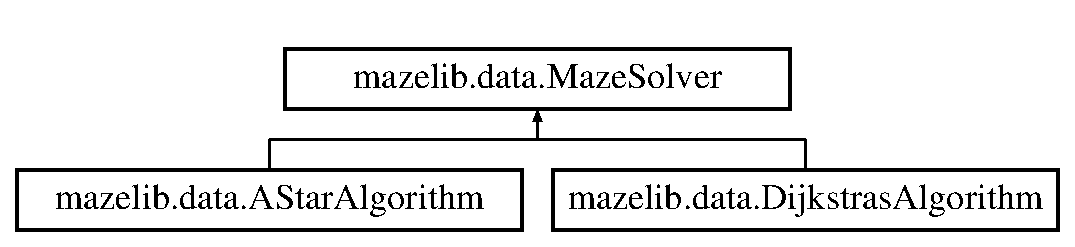
\includegraphics[height=2.000000cm]{classmazelib_1_1data_1_1_maze_solver}
\end{center}
\end{figure}
\subsection*{Public Member Functions}
\begin{DoxyCompactItemize}
\item 
\hyperlink{classmazelib_1_1data_1_1_maze_solver_a9d109ec788a834fb4af13e8d15690c1f}{Maze\-Solver} (\hyperlink{classmazelib_1_1data_1_1_maze}{Maze} maze, \hyperlink{interfacemazelib_1_1data_1_1_heuristic}{Heuristic} heuristic)
\item 
\hyperlink{classmazelib_1_1data_1_1_maze_solver_a45b8264a170235e86e9e2d304670d090}{Maze\-Solver} (String string\-Maze, \hyperlink{interfacemazelib_1_1data_1_1_heuristic}{Heuristic} heuristic)
\item 
abstract List$<$ \hyperlink{classmazelib_1_1data_1_1_node}{Node} $>$ \hyperlink{classmazelib_1_1data_1_1_maze_solver_a009bd983cdccfb7c845d3da8fabf02d6}{solve\-Maze} ()
\item 
String \hyperlink{classmazelib_1_1data_1_1_maze_solver_a314017420b6dc62fff186502d7e21dc2}{draw\-Solution} ()
\end{DoxyCompactItemize}
\subsection*{Protected Attributes}
\begin{DoxyCompactItemize}
\item 
\hypertarget{classmazelib_1_1data_1_1_maze_solver_ade82d3652ee86f02ff0f16f8ddff5ea0}{\hyperlink{classmazelib_1_1data_1_1_maze}{Maze} {\bfseries maze}}\label{classmazelib_1_1data_1_1_maze_solver_ade82d3652ee86f02ff0f16f8ddff5ea0}

\item 
\hypertarget{classmazelib_1_1data_1_1_maze_solver_a8f57c9e54a2e368c429b11c5ba7707af}{final \hyperlink{interfacemazelib_1_1data_1_1_heuristic}{Heuristic} {\bfseries heuristic}}\label{classmazelib_1_1data_1_1_maze_solver_a8f57c9e54a2e368c429b11c5ba7707af}

\item 
\hypertarget{classmazelib_1_1data_1_1_maze_solver_a089ceaab209320b6df17dd27f4d58eae}{Map$<$ \hyperlink{classmazelib_1_1data_1_1_node}{Node}, Boolean $>$ {\bfseries solution\-Nodes}}\label{classmazelib_1_1data_1_1_maze_solver_a089ceaab209320b6df17dd27f4d58eae}

\item 
\hypertarget{classmazelib_1_1data_1_1_maze_solver_ac6f12a1f0ad8e35ffae101a5ec7cabfd}{final long {\bfseries C\-O\-S\-T\-\_\-\-S\-T\-R\-A\-I\-G\-H\-T} = 100l}\label{classmazelib_1_1data_1_1_maze_solver_ac6f12a1f0ad8e35ffae101a5ec7cabfd}

\item 
\hypertarget{classmazelib_1_1data_1_1_maze_solver_a161ad7fae780c4e07703d87508657304}{final long {\bfseries C\-O\-S\-T\-\_\-\-D\-I\-A\-G\-O\-N\-A\-L} = 141l}\label{classmazelib_1_1data_1_1_maze_solver_a161ad7fae780c4e07703d87508657304}

\end{DoxyCompactItemize}


\subsection{Detailed Description}
Template method for \hyperlink{classmazelib_1_1data_1_1_maze}{Maze} solving algorithms \begin{DoxyAuthor}{Author}
Timur Reziapov \href{mailto:reziapo1@illinois.edu}{\tt reziapo1@illinois.\-edu} 
\end{DoxyAuthor}
\begin{DoxyDate}{Date}
Wednesday, September 5, 2012 15\-:00 P\-M 
\end{DoxyDate}


\subsection{Constructor \& Destructor Documentation}
\hypertarget{classmazelib_1_1data_1_1_maze_solver_a9d109ec788a834fb4af13e8d15690c1f}{\index{mazelib\-::data\-::\-Maze\-Solver@{mazelib\-::data\-::\-Maze\-Solver}!Maze\-Solver@{Maze\-Solver}}
\index{Maze\-Solver@{Maze\-Solver}!mazelib::data::MazeSolver@{mazelib\-::data\-::\-Maze\-Solver}}
\subsubsection[{Maze\-Solver}]{\setlength{\rightskip}{0pt plus 5cm}mazelib.\-data.\-Maze\-Solver.\-Maze\-Solver (
\begin{DoxyParamCaption}
\item[{{\bf Maze}}]{maze, }
\item[{{\bf Heuristic}}]{heuristic}
\end{DoxyParamCaption}
)\hspace{0.3cm}{\ttfamily [inline]}}}\label{classmazelib_1_1data_1_1_maze_solver_a9d109ec788a834fb4af13e8d15690c1f}
Constructor to be used by derived classes. 
\begin{DoxyParams}{Parameters}
{\em maze} & the \hyperlink{classmazelib_1_1data_1_1_maze}{Maze} to work on \\
\hline
\end{DoxyParams}
\hypertarget{classmazelib_1_1data_1_1_maze_solver_a45b8264a170235e86e9e2d304670d090}{\index{mazelib\-::data\-::\-Maze\-Solver@{mazelib\-::data\-::\-Maze\-Solver}!Maze\-Solver@{Maze\-Solver}}
\index{Maze\-Solver@{Maze\-Solver}!mazelib::data::MazeSolver@{mazelib\-::data\-::\-Maze\-Solver}}
\subsubsection[{Maze\-Solver}]{\setlength{\rightskip}{0pt plus 5cm}mazelib.\-data.\-Maze\-Solver.\-Maze\-Solver (
\begin{DoxyParamCaption}
\item[{String}]{string\-Maze, }
\item[{{\bf Heuristic}}]{heuristic}
\end{DoxyParamCaption}
)\hspace{0.3cm}{\ttfamily [inline]}}}\label{classmazelib_1_1data_1_1_maze_solver_a45b8264a170235e86e9e2d304670d090}
Constructor to be used by derived classes. 
\begin{DoxyParams}{Parameters}
{\em string\-Maze} & the string representation of the \hyperlink{classmazelib_1_1data_1_1_maze}{Maze} to solve \\
\hline
\end{DoxyParams}


\subsection{Member Function Documentation}
\hypertarget{classmazelib_1_1data_1_1_maze_solver_a314017420b6dc62fff186502d7e21dc2}{\index{mazelib\-::data\-::\-Maze\-Solver@{mazelib\-::data\-::\-Maze\-Solver}!draw\-Solution@{draw\-Solution}}
\index{draw\-Solution@{draw\-Solution}!mazelib::data::MazeSolver@{mazelib\-::data\-::\-Maze\-Solver}}
\subsubsection[{draw\-Solution}]{\setlength{\rightskip}{0pt plus 5cm}String mazelib.\-data.\-Maze\-Solver.\-draw\-Solution (
\begin{DoxyParamCaption}
{}
\end{DoxyParamCaption}
)\hspace{0.3cm}{\ttfamily [inline]}}}\label{classmazelib_1_1data_1_1_maze_solver_a314017420b6dc62fff186502d7e21dc2}
This function draws the maze with solution path. \begin{DoxyReturn}{Returns}
the string representation of \hyperlink{classmazelib_1_1data_1_1_maze}{Maze} with solution path, null if \hyperlink{classmazelib_1_1data_1_1_maze}{Maze} hasn't been solved yet 
\end{DoxyReturn}
\hypertarget{classmazelib_1_1data_1_1_maze_solver_a009bd983cdccfb7c845d3da8fabf02d6}{\index{mazelib\-::data\-::\-Maze\-Solver@{mazelib\-::data\-::\-Maze\-Solver}!solve\-Maze@{solve\-Maze}}
\index{solve\-Maze@{solve\-Maze}!mazelib::data::MazeSolver@{mazelib\-::data\-::\-Maze\-Solver}}
\subsubsection[{solve\-Maze}]{\setlength{\rightskip}{0pt plus 5cm}abstract List$<${\bf Node}$>$ mazelib.\-data.\-Maze\-Solver.\-solve\-Maze (
\begin{DoxyParamCaption}
{}
\end{DoxyParamCaption}
)\hspace{0.3cm}{\ttfamily [pure virtual]}}}\label{classmazelib_1_1data_1_1_maze_solver_a009bd983cdccfb7c845d3da8fabf02d6}
Main algorithm method that each non-\/abstract derived class must define. \begin{DoxyReturn}{Returns}
the List of solution Nodes 
\end{DoxyReturn}


Implemented in \hyperlink{classmazelib_1_1data_1_1_a_star_algorithm_aaa690f9111cf47f54a10c84c28cfcba4}{mazelib.\-data.\-A\-Star\-Algorithm}, and \hyperlink{classmazelib_1_1data_1_1_dijkstras_algorithm_abe1208942d2a0397235aef4737990ca2}{mazelib.\-data.\-Dijkstras\-Algorithm}.



The documentation for this class was generated from the following file\-:\begin{DoxyCompactItemize}
\item 
src/mazelib/data/Maze\-Solver.\-java\end{DoxyCompactItemize}

\hypertarget{classmazelib_1_1tests_1_1_maze_test}{\section{mazelib.\-tests.\-Maze\-Test Class Reference}
\label{classmazelib_1_1tests_1_1_maze_test}\index{mazelib.\-tests.\-Maze\-Test@{mazelib.\-tests.\-Maze\-Test}}
}
\subsection*{Public Member Functions}
\begin{DoxyCompactItemize}
\item 
void \hyperlink{classmazelib_1_1tests_1_1_maze_test_ab0b2a3fb6a31b1e842ec2426f6ec25ba}{test\-Initialization} ()
\item 
void \hyperlink{classmazelib_1_1tests_1_1_maze_test_ab8f188842ecb12b90a27d06e642d6d5e}{test\-Illegal\-Maze} ()
\item 
void \hyperlink{classmazelib_1_1tests_1_1_maze_test_a27e62c8b2f0353746a4e2a1b13e1d4d2}{test\-Get\-Node} ()
\item 
void \hyperlink{classmazelib_1_1tests_1_1_maze_test_a9a8950ef982e1dea795f7fd772b6d606}{test\-Perfect\-Maze} ()
\item 
void \hyperlink{classmazelib_1_1tests_1_1_maze_test_ab716c61475125c279f10adc0098fc33f}{test\-Draw\-Maze} ()
\item 
void \hyperlink{classmazelib_1_1tests_1_1_maze_test_a662f324e8321096a6087f8d44a9479d0}{test\-String\-Constructor} ()
\end{DoxyCompactItemize}
\subsection*{Static Public Member Functions}
\begin{DoxyCompactItemize}
\item 
static void \hyperlink{classmazelib_1_1tests_1_1_maze_test_aa190b5be34fedf99a6d49df89e797d67}{set\-Up\-Before\-Class} ()  throws Exception  	
\end{DoxyCompactItemize}


\subsection{Detailed Description}
\begin{DoxyAuthor}{Author}
Timur Reziapov \href{mailto:reziapo1@illinois.edu}{\tt reziapo1@illinois.\-edu} 
\end{DoxyAuthor}
\begin{DoxyDate}{Date}
Monday, September 3, 2012, 18\-:00 P\-M 
\end{DoxyDate}


\subsection{Member Function Documentation}
\hypertarget{classmazelib_1_1tests_1_1_maze_test_aa190b5be34fedf99a6d49df89e797d67}{\index{mazelib\-::tests\-::\-Maze\-Test@{mazelib\-::tests\-::\-Maze\-Test}!set\-Up\-Before\-Class@{set\-Up\-Before\-Class}}
\index{set\-Up\-Before\-Class@{set\-Up\-Before\-Class}!mazelib::tests::MazeTest@{mazelib\-::tests\-::\-Maze\-Test}}
\subsubsection[{set\-Up\-Before\-Class}]{\setlength{\rightskip}{0pt plus 5cm}static void mazelib.\-tests.\-Maze\-Test.\-set\-Up\-Before\-Class (
\begin{DoxyParamCaption}
{}
\end{DoxyParamCaption}
)  throws Exception  	\hspace{0.3cm}{\ttfamily [inline]}, {\ttfamily [static]}}}\label{classmazelib_1_1tests_1_1_maze_test_aa190b5be34fedf99a6d49df89e797d67}
This test is run before any other tests. 
\begin{DoxyExceptions}{Exceptions}
{\em Exception} & \\
\hline
\end{DoxyExceptions}
\hypertarget{classmazelib_1_1tests_1_1_maze_test_ab716c61475125c279f10adc0098fc33f}{\index{mazelib\-::tests\-::\-Maze\-Test@{mazelib\-::tests\-::\-Maze\-Test}!test\-Draw\-Maze@{test\-Draw\-Maze}}
\index{test\-Draw\-Maze@{test\-Draw\-Maze}!mazelib::tests::MazeTest@{mazelib\-::tests\-::\-Maze\-Test}}
\subsubsection[{test\-Draw\-Maze}]{\setlength{\rightskip}{0pt plus 5cm}void mazelib.\-tests.\-Maze\-Test.\-test\-Draw\-Maze (
\begin{DoxyParamCaption}
{}
\end{DoxyParamCaption}
)\hspace{0.3cm}{\ttfamily [inline]}}}\label{classmazelib_1_1tests_1_1_maze_test_ab716c61475125c279f10adc0098fc33f}
This test to see if draw\-Maze correctly represents a maze as a String, and if the same maze is drawn the same way twice. \hypertarget{classmazelib_1_1tests_1_1_maze_test_a27e62c8b2f0353746a4e2a1b13e1d4d2}{\index{mazelib\-::tests\-::\-Maze\-Test@{mazelib\-::tests\-::\-Maze\-Test}!test\-Get\-Node@{test\-Get\-Node}}
\index{test\-Get\-Node@{test\-Get\-Node}!mazelib::tests::MazeTest@{mazelib\-::tests\-::\-Maze\-Test}}
\subsubsection[{test\-Get\-Node}]{\setlength{\rightskip}{0pt plus 5cm}void mazelib.\-tests.\-Maze\-Test.\-test\-Get\-Node (
\begin{DoxyParamCaption}
{}
\end{DoxyParamCaption}
)\hspace{0.3cm}{\ttfamily [inline]}}}\label{classmazelib_1_1tests_1_1_maze_test_a27e62c8b2f0353746a4e2a1b13e1d4d2}
Test to check if get\-Node returns the correct Node and handles Positions out of bounds properly. Indirectly tests in\-Bounds. \hypertarget{classmazelib_1_1tests_1_1_maze_test_ab8f188842ecb12b90a27d06e642d6d5e}{\index{mazelib\-::tests\-::\-Maze\-Test@{mazelib\-::tests\-::\-Maze\-Test}!test\-Illegal\-Maze@{test\-Illegal\-Maze}}
\index{test\-Illegal\-Maze@{test\-Illegal\-Maze}!mazelib::tests::MazeTest@{mazelib\-::tests\-::\-Maze\-Test}}
\subsubsection[{test\-Illegal\-Maze}]{\setlength{\rightskip}{0pt plus 5cm}void mazelib.\-tests.\-Maze\-Test.\-test\-Illegal\-Maze (
\begin{DoxyParamCaption}
{}
\end{DoxyParamCaption}
)\hspace{0.3cm}{\ttfamily [inline]}}}\label{classmazelib_1_1tests_1_1_maze_test_ab8f188842ecb12b90a27d06e642d6d5e}
Test illegal Maze creation. \hypertarget{classmazelib_1_1tests_1_1_maze_test_ab0b2a3fb6a31b1e842ec2426f6ec25ba}{\index{mazelib\-::tests\-::\-Maze\-Test@{mazelib\-::tests\-::\-Maze\-Test}!test\-Initialization@{test\-Initialization}}
\index{test\-Initialization@{test\-Initialization}!mazelib::tests::MazeTest@{mazelib\-::tests\-::\-Maze\-Test}}
\subsubsection[{test\-Initialization}]{\setlength{\rightskip}{0pt plus 5cm}void mazelib.\-tests.\-Maze\-Test.\-test\-Initialization (
\begin{DoxyParamCaption}
{}
\end{DoxyParamCaption}
)\hspace{0.3cm}{\ttfamily [inline]}}}\label{classmazelib_1_1tests_1_1_maze_test_ab0b2a3fb6a31b1e842ec2426f6ec25ba}
This test checks if a Maze has been properly initialized. \hypertarget{classmazelib_1_1tests_1_1_maze_test_a9a8950ef982e1dea795f7fd772b6d606}{\index{mazelib\-::tests\-::\-Maze\-Test@{mazelib\-::tests\-::\-Maze\-Test}!test\-Perfect\-Maze@{test\-Perfect\-Maze}}
\index{test\-Perfect\-Maze@{test\-Perfect\-Maze}!mazelib::tests::MazeTest@{mazelib\-::tests\-::\-Maze\-Test}}
\subsubsection[{test\-Perfect\-Maze}]{\setlength{\rightskip}{0pt plus 5cm}void mazelib.\-tests.\-Maze\-Test.\-test\-Perfect\-Maze (
\begin{DoxyParamCaption}
{}
\end{DoxyParamCaption}
)\hspace{0.3cm}{\ttfamily [inline]}}}\label{classmazelib_1_1tests_1_1_maze_test_a9a8950ef982e1dea795f7fd772b6d606}
This test is used to check if the random Maze paths were generated by checking if its a perfect Maze\-: specifically all passable Nodes are reachable from start, i.\-e. traversable. Basically requires full functionality of both Node and Maze classes. \hypertarget{classmazelib_1_1tests_1_1_maze_test_a662f324e8321096a6087f8d44a9479d0}{\index{mazelib\-::tests\-::\-Maze\-Test@{mazelib\-::tests\-::\-Maze\-Test}!test\-String\-Constructor@{test\-String\-Constructor}}
\index{test\-String\-Constructor@{test\-String\-Constructor}!mazelib::tests::MazeTest@{mazelib\-::tests\-::\-Maze\-Test}}
\subsubsection[{test\-String\-Constructor}]{\setlength{\rightskip}{0pt plus 5cm}void mazelib.\-tests.\-Maze\-Test.\-test\-String\-Constructor (
\begin{DoxyParamCaption}
{}
\end{DoxyParamCaption}
)\hspace{0.3cm}{\ttfamily [inline]}}}\label{classmazelib_1_1tests_1_1_maze_test_a662f324e8321096a6087f8d44a9479d0}
This test checks if a Maze can be generated using the string constructor. 

The documentation for this class was generated from the following file\-:\begin{DoxyCompactItemize}
\item 
src/mazelib/tests/Maze\-Test.\-java\end{DoxyCompactItemize}

\hypertarget{classmazelib_1_1data_1_1_node}{\section{mazelib.\-data.\-Node Class Reference}
\label{classmazelib_1_1data_1_1_node}\index{mazelib.\-data.\-Node@{mazelib.\-data.\-Node}}
}
Inheritance diagram for mazelib.\-data.\-Node\-:\begin{figure}[H]
\begin{center}
\leavevmode
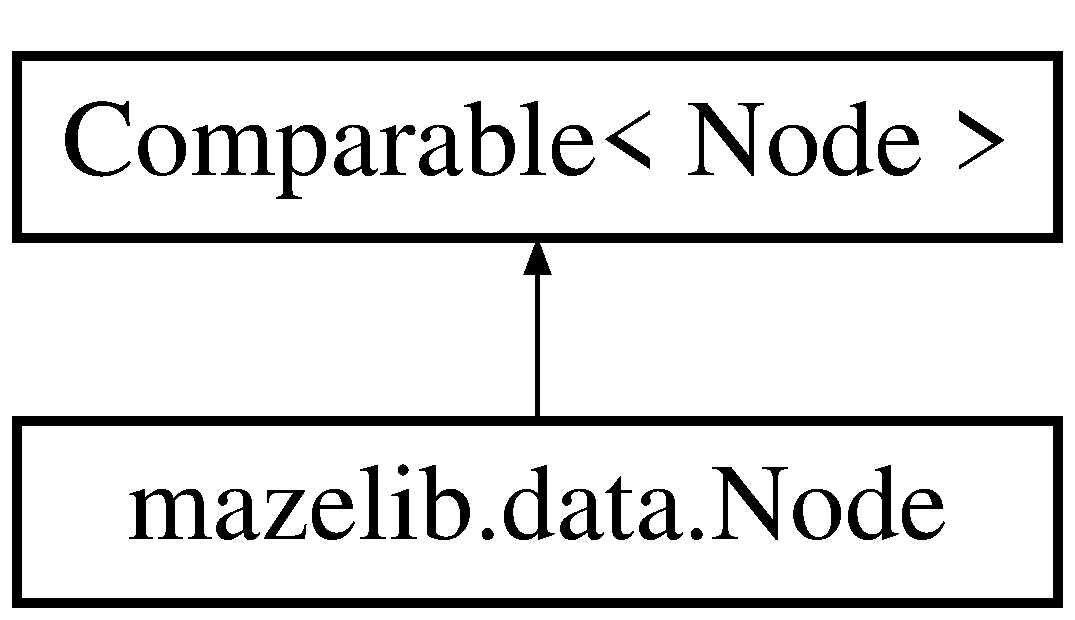
\includegraphics[height=2.000000cm]{classmazelib_1_1data_1_1_node}
\end{center}
\end{figure}
\subsection*{Public Member Functions}
\begin{DoxyCompactItemize}
\item 
int \hyperlink{classmazelib_1_1data_1_1_node_a6d0332471e8e795262b54c42a7f72cd3}{compare\-To} (\hyperlink{classmazelib_1_1data_1_1_node}{Node} other)
\item 
List$<$ \hyperlink{classmazelib_1_1data_1_1_node}{Node} $>$ \hyperlink{classmazelib_1_1data_1_1_node_a7f1c31cd172078f0d2160639ceae4d6c}{get\-Adjacent\-Nodes} (boolean diagonal)
\item 
boolean \hyperlink{classmazelib_1_1data_1_1_node_abbb9f4db2a23abe1b5ab79aabf632c9c}{can\-Reach} (\hyperlink{classmazelib_1_1data_1_1_node}{Node} neighbor\-Node)
\item 
long \hyperlink{classmazelib_1_1data_1_1_node_a2ad7aa3cd7165ffff7634ebf6e362549}{get\-Accumulated\-Cost} ()
\item 
void \hyperlink{classmazelib_1_1data_1_1_node_a74f88136c6d4c5953db07872b951ae4b}{set\-Accumulated\-Cost} (long accumulated\-Cost)
\item 
long \hyperlink{classmazelib_1_1data_1_1_node_a3e9f05a1e91e8bc6879c2f600e819d7b}{get\-Estimated\-Cost} ()
\item 
void \hyperlink{classmazelib_1_1data_1_1_node_a8405b28d885d50e4bcfa4ef21c5f0942}{set\-Estimated\-Cost} (long estimated\-Cost)
\item 
long \hyperlink{classmazelib_1_1data_1_1_node_a1cc1fcda8a17f24bc72f810c0f76b02e}{get\-Total\-Cost} ()
\item 
\hyperlink{classmazelib_1_1data_1_1_node}{Node} \hyperlink{classmazelib_1_1data_1_1_node_a320a1eae56bbede15573be0499556465}{get\-Parent\-Node} ()
\item 
void \hyperlink{classmazelib_1_1data_1_1_node_a1da6285dea279ef17d514cc8a8f8cbfd}{set\-Parent\-Node} (\hyperlink{classmazelib_1_1data_1_1_node}{Node} parent\-Node)
\item 
\hyperlink{classmazelib_1_1data_1_1_position}{Position} \hyperlink{classmazelib_1_1data_1_1_node_acb069d8e4430f951bebe4c0188e222bc}{get\-Position} ()
\item 
boolean \hyperlink{classmazelib_1_1data_1_1_node_aa54c4931c5ae776275ea2b9128858eec}{get\-Is\-Passable} ()
\item 
\hyperlink{classmazelib_1_1data_1_1_maze}{Maze} \hyperlink{classmazelib_1_1data_1_1_node_aafef828ac17d63ff39d0ae27cf2d761d}{get\-Parent\-Maze} ()
\item 
int \hyperlink{classmazelib_1_1data_1_1_node_a9ff18335087c35e4b6fa7b9796f5f7ef}{hash\-Code} ()
\item 
boolean \hyperlink{classmazelib_1_1data_1_1_node_a5921df3fa5ccb2c3ff328039f7924b93}{equals} (Object other)
\end{DoxyCompactItemize}
\subsection*{Protected Member Functions}
\begin{DoxyCompactItemize}
\item 
\hyperlink{classmazelib_1_1data_1_1_node_abb9bb1179d4fa3877d267126a72146fd}{Node} (\hyperlink{classmazelib_1_1data_1_1_position}{Position} position, boolean passable, \hyperlink{classmazelib_1_1data_1_1_maze}{Maze} parent\-Maze)
\item 
void \hyperlink{classmazelib_1_1data_1_1_node_a0e95a8e452791ec769b56bb7d5cf2132}{set\-Passable} (boolean passable)
\end{DoxyCompactItemize}


\subsection{Detailed Description}
This class represents a block in a \hyperlink{classmazelib_1_1data_1_1_maze}{Maze}. \begin{DoxyAuthor}{Author}
Timur Reziapov \href{mailto:reziapo1@illinois.edu}{\tt reziapo1@illinois.\-edu} 
\end{DoxyAuthor}
\begin{DoxyDate}{Date}
Sunday, September 2, 2012 17\-:00 P\-M 
\end{DoxyDate}


\subsection{Constructor \& Destructor Documentation}
\hypertarget{classmazelib_1_1data_1_1_node_abb9bb1179d4fa3877d267126a72146fd}{\index{mazelib\-::data\-::\-Node@{mazelib\-::data\-::\-Node}!Node@{Node}}
\index{Node@{Node}!mazelib::data::Node@{mazelib\-::data\-::\-Node}}
\subsubsection[{Node}]{\setlength{\rightskip}{0pt plus 5cm}mazelib.\-data.\-Node.\-Node (
\begin{DoxyParamCaption}
\item[{{\bf Position}}]{position, }
\item[{boolean}]{passable, }
\item[{{\bf Maze}}]{parent\-Maze}
\end{DoxyParamCaption}
)\hspace{0.3cm}{\ttfamily [inline]}, {\ttfamily [protected]}}}\label{classmazelib_1_1data_1_1_node_abb9bb1179d4fa3877d267126a72146fd}
Constructs a \hyperlink{classmazelib_1_1data_1_1_node}{Node}. Protected because we only want to allow creation of Nodes from within a \hyperlink{classmazelib_1_1data_1_1_maze}{Maze} object. 
\begin{DoxyParams}{Parameters}
{\em position} & the \hyperlink{classmazelib_1_1data_1_1_position}{Position} of \hyperlink{classmazelib_1_1data_1_1_node}{Node} in a \hyperlink{classmazelib_1_1data_1_1_maze}{Maze} \\
\hline
{\em passable} & determines if \hyperlink{classmazelib_1_1data_1_1_node}{Node} is a wall or not \\
\hline
\end{DoxyParams}


\subsection{Member Function Documentation}
\hypertarget{classmazelib_1_1data_1_1_node_abbb9f4db2a23abe1b5ab79aabf632c9c}{\index{mazelib\-::data\-::\-Node@{mazelib\-::data\-::\-Node}!can\-Reach@{can\-Reach}}
\index{can\-Reach@{can\-Reach}!mazelib::data::Node@{mazelib\-::data\-::\-Node}}
\subsubsection[{can\-Reach}]{\setlength{\rightskip}{0pt plus 5cm}boolean mazelib.\-data.\-Node.\-can\-Reach (
\begin{DoxyParamCaption}
\item[{{\bf Node}}]{neighbor\-Node}
\end{DoxyParamCaption}
)\hspace{0.3cm}{\ttfamily [inline]}}}\label{classmazelib_1_1data_1_1_node_abbb9f4db2a23abe1b5ab79aabf632c9c}
Function to check if target\-Node is reachable from this \hyperlink{classmazelib_1_1data_1_1_node}{Node}. 
\begin{DoxyParams}{Parameters}
{\em target\-Node} & the \hyperlink{classmazelib_1_1data_1_1_node}{Node} to check reaching to \\
\hline
\end{DoxyParams}
\begin{DoxyReturn}{Returns}
true if target \hyperlink{classmazelib_1_1data_1_1_node}{Node} is reachable from this \hyperlink{classmazelib_1_1data_1_1_node}{Node}, false otherwise 
\end{DoxyReturn}
\hypertarget{classmazelib_1_1data_1_1_node_a6d0332471e8e795262b54c42a7f72cd3}{\index{mazelib\-::data\-::\-Node@{mazelib\-::data\-::\-Node}!compare\-To@{compare\-To}}
\index{compare\-To@{compare\-To}!mazelib::data::Node@{mazelib\-::data\-::\-Node}}
\subsubsection[{compare\-To}]{\setlength{\rightskip}{0pt plus 5cm}int mazelib.\-data.\-Node.\-compare\-To (
\begin{DoxyParamCaption}
\item[{{\bf Node}}]{other}
\end{DoxyParamCaption}
)\hspace{0.3cm}{\ttfamily [inline]}}}\label{classmazelib_1_1data_1_1_node_a6d0332471e8e795262b54c42a7f72cd3}
other \hyperlink{classmazelib_1_1data_1_1_node}{Node} is from the same parent \hyperlink{classmazelib_1_1data_1_1_maze}{Maze} \begin{DoxyReturn}{Returns}
1 if this \hyperlink{classmazelib_1_1data_1_1_node}{Node} has a higher total cost than parameter \hyperlink{classmazelib_1_1data_1_1_node}{Node}, 0 if this \hyperlink{classmazelib_1_1data_1_1_node}{Node} and parameter \hyperlink{classmazelib_1_1data_1_1_node}{Node} have the same total cost, and -\/1 if this \hyperlink{classmazelib_1_1data_1_1_node}{Node} has a smaller total cost than parameter \hyperlink{classmazelib_1_1data_1_1_node}{Node}. 
\end{DoxyReturn}
\hypertarget{classmazelib_1_1data_1_1_node_a5921df3fa5ccb2c3ff328039f7924b93}{\index{mazelib\-::data\-::\-Node@{mazelib\-::data\-::\-Node}!equals@{equals}}
\index{equals@{equals}!mazelib::data::Node@{mazelib\-::data\-::\-Node}}
\subsubsection[{equals}]{\setlength{\rightskip}{0pt plus 5cm}boolean mazelib.\-data.\-Node.\-equals (
\begin{DoxyParamCaption}
\item[{Object}]{other}
\end{DoxyParamCaption}
)\hspace{0.3cm}{\ttfamily [inline]}}}\label{classmazelib_1_1data_1_1_node_a5921df3fa5ccb2c3ff328039f7924b93}
\begin{DoxyReturn}{Returns}
true if other is a \hyperlink{classmazelib_1_1data_1_1_node}{Node} with equal fields false otherwise 
\end{DoxyReturn}
\hypertarget{classmazelib_1_1data_1_1_node_a2ad7aa3cd7165ffff7634ebf6e362549}{\index{mazelib\-::data\-::\-Node@{mazelib\-::data\-::\-Node}!get\-Accumulated\-Cost@{get\-Accumulated\-Cost}}
\index{get\-Accumulated\-Cost@{get\-Accumulated\-Cost}!mazelib::data::Node@{mazelib\-::data\-::\-Node}}
\subsubsection[{get\-Accumulated\-Cost}]{\setlength{\rightskip}{0pt plus 5cm}long mazelib.\-data.\-Node.\-get\-Accumulated\-Cost (
\begin{DoxyParamCaption}
{}
\end{DoxyParamCaption}
)\hspace{0.3cm}{\ttfamily [inline]}}}\label{classmazelib_1_1data_1_1_node_a2ad7aa3cd7165ffff7634ebf6e362549}
\begin{DoxyReturn}{Returns}
the accumulated cost for this \hyperlink{classmazelib_1_1data_1_1_node}{Node} 
\end{DoxyReturn}
\hypertarget{classmazelib_1_1data_1_1_node_a7f1c31cd172078f0d2160639ceae4d6c}{\index{mazelib\-::data\-::\-Node@{mazelib\-::data\-::\-Node}!get\-Adjacent\-Nodes@{get\-Adjacent\-Nodes}}
\index{get\-Adjacent\-Nodes@{get\-Adjacent\-Nodes}!mazelib::data::Node@{mazelib\-::data\-::\-Node}}
\subsubsection[{get\-Adjacent\-Nodes}]{\setlength{\rightskip}{0pt plus 5cm}List$<${\bf Node}$>$ mazelib.\-data.\-Node.\-get\-Adjacent\-Nodes (
\begin{DoxyParamCaption}
\item[{boolean}]{diagonal}
\end{DoxyParamCaption}
)\hspace{0.3cm}{\ttfamily [inline]}}}\label{classmazelib_1_1data_1_1_node_a7f1c31cd172078f0d2160639ceae4d6c}
This function is used to get this \hyperlink{classmazelib_1_1data_1_1_node}{Node}'s adjacent Nodes. 
\begin{DoxyParams}{Parameters}
{\em diagonal} & whether to include or not diagonal neighbors in return \\
\hline
\end{DoxyParams}
\begin{DoxyReturn}{Returns}
the list of non-\/diagonal adjacent Nodes 
\end{DoxyReturn}
\hypertarget{classmazelib_1_1data_1_1_node_a3e9f05a1e91e8bc6879c2f600e819d7b}{\index{mazelib\-::data\-::\-Node@{mazelib\-::data\-::\-Node}!get\-Estimated\-Cost@{get\-Estimated\-Cost}}
\index{get\-Estimated\-Cost@{get\-Estimated\-Cost}!mazelib::data::Node@{mazelib\-::data\-::\-Node}}
\subsubsection[{get\-Estimated\-Cost}]{\setlength{\rightskip}{0pt plus 5cm}long mazelib.\-data.\-Node.\-get\-Estimated\-Cost (
\begin{DoxyParamCaption}
{}
\end{DoxyParamCaption}
)\hspace{0.3cm}{\ttfamily [inline]}}}\label{classmazelib_1_1data_1_1_node_a3e9f05a1e91e8bc6879c2f600e819d7b}
\begin{DoxyReturn}{Returns}
the estimated cost for this \hyperlink{classmazelib_1_1data_1_1_node}{Node} 
\end{DoxyReturn}
\hypertarget{classmazelib_1_1data_1_1_node_aa54c4931c5ae776275ea2b9128858eec}{\index{mazelib\-::data\-::\-Node@{mazelib\-::data\-::\-Node}!get\-Is\-Passable@{get\-Is\-Passable}}
\index{get\-Is\-Passable@{get\-Is\-Passable}!mazelib::data::Node@{mazelib\-::data\-::\-Node}}
\subsubsection[{get\-Is\-Passable}]{\setlength{\rightskip}{0pt plus 5cm}boolean mazelib.\-data.\-Node.\-get\-Is\-Passable (
\begin{DoxyParamCaption}
{}
\end{DoxyParamCaption}
)\hspace{0.3cm}{\ttfamily [inline]}}}\label{classmazelib_1_1data_1_1_node_aa54c4931c5ae776275ea2b9128858eec}
\begin{DoxyReturn}{Returns}
if this \hyperlink{classmazelib_1_1data_1_1_node}{Node} is passable or impassable 
\end{DoxyReturn}
\hypertarget{classmazelib_1_1data_1_1_node_aafef828ac17d63ff39d0ae27cf2d761d}{\index{mazelib\-::data\-::\-Node@{mazelib\-::data\-::\-Node}!get\-Parent\-Maze@{get\-Parent\-Maze}}
\index{get\-Parent\-Maze@{get\-Parent\-Maze}!mazelib::data::Node@{mazelib\-::data\-::\-Node}}
\subsubsection[{get\-Parent\-Maze}]{\setlength{\rightskip}{0pt plus 5cm}{\bf Maze} mazelib.\-data.\-Node.\-get\-Parent\-Maze (
\begin{DoxyParamCaption}
{}
\end{DoxyParamCaption}
)\hspace{0.3cm}{\ttfamily [inline]}}}\label{classmazelib_1_1data_1_1_node_aafef828ac17d63ff39d0ae27cf2d761d}
\begin{DoxyReturn}{Returns}
the parent \hyperlink{classmazelib_1_1data_1_1_maze}{Maze} of this \hyperlink{classmazelib_1_1data_1_1_node}{Node} 
\end{DoxyReturn}
\hypertarget{classmazelib_1_1data_1_1_node_a320a1eae56bbede15573be0499556465}{\index{mazelib\-::data\-::\-Node@{mazelib\-::data\-::\-Node}!get\-Parent\-Node@{get\-Parent\-Node}}
\index{get\-Parent\-Node@{get\-Parent\-Node}!mazelib::data::Node@{mazelib\-::data\-::\-Node}}
\subsubsection[{get\-Parent\-Node}]{\setlength{\rightskip}{0pt plus 5cm}{\bf Node} mazelib.\-data.\-Node.\-get\-Parent\-Node (
\begin{DoxyParamCaption}
{}
\end{DoxyParamCaption}
)\hspace{0.3cm}{\ttfamily [inline]}}}\label{classmazelib_1_1data_1_1_node_a320a1eae56bbede15573be0499556465}
\begin{DoxyReturn}{Returns}
the parent \hyperlink{classmazelib_1_1data_1_1_node}{Node} of this \hyperlink{classmazelib_1_1data_1_1_node}{Node} 
\end{DoxyReturn}
\hypertarget{classmazelib_1_1data_1_1_node_acb069d8e4430f951bebe4c0188e222bc}{\index{mazelib\-::data\-::\-Node@{mazelib\-::data\-::\-Node}!get\-Position@{get\-Position}}
\index{get\-Position@{get\-Position}!mazelib::data::Node@{mazelib\-::data\-::\-Node}}
\subsubsection[{get\-Position}]{\setlength{\rightskip}{0pt plus 5cm}{\bf Position} mazelib.\-data.\-Node.\-get\-Position (
\begin{DoxyParamCaption}
{}
\end{DoxyParamCaption}
)\hspace{0.3cm}{\ttfamily [inline]}}}\label{classmazelib_1_1data_1_1_node_acb069d8e4430f951bebe4c0188e222bc}
\begin{DoxyReturn}{Returns}
the \hyperlink{classmazelib_1_1data_1_1_position}{Position} of this \hyperlink{classmazelib_1_1data_1_1_node}{Node} 
\end{DoxyReturn}
\hypertarget{classmazelib_1_1data_1_1_node_a1cc1fcda8a17f24bc72f810c0f76b02e}{\index{mazelib\-::data\-::\-Node@{mazelib\-::data\-::\-Node}!get\-Total\-Cost@{get\-Total\-Cost}}
\index{get\-Total\-Cost@{get\-Total\-Cost}!mazelib::data::Node@{mazelib\-::data\-::\-Node}}
\subsubsection[{get\-Total\-Cost}]{\setlength{\rightskip}{0pt plus 5cm}long mazelib.\-data.\-Node.\-get\-Total\-Cost (
\begin{DoxyParamCaption}
{}
\end{DoxyParamCaption}
)\hspace{0.3cm}{\ttfamily [inline]}}}\label{classmazelib_1_1data_1_1_node_a1cc1fcda8a17f24bc72f810c0f76b02e}
\begin{DoxyReturn}{Returns}
total cost of this \hyperlink{classmazelib_1_1data_1_1_node}{Node} 
\end{DoxyReturn}
\hypertarget{classmazelib_1_1data_1_1_node_a9ff18335087c35e4b6fa7b9796f5f7ef}{\index{mazelib\-::data\-::\-Node@{mazelib\-::data\-::\-Node}!hash\-Code@{hash\-Code}}
\index{hash\-Code@{hash\-Code}!mazelib::data::Node@{mazelib\-::data\-::\-Node}}
\subsubsection[{hash\-Code}]{\setlength{\rightskip}{0pt plus 5cm}int mazelib.\-data.\-Node.\-hash\-Code (
\begin{DoxyParamCaption}
{}
\end{DoxyParamCaption}
)\hspace{0.3cm}{\ttfamily [inline]}}}\label{classmazelib_1_1data_1_1_node_a9ff18335087c35e4b6fa7b9796f5f7ef}
Returns an integer that corresponds to this \hyperlink{classmazelib_1_1data_1_1_node}{Node}'s \hyperlink{classmazelib_1_1data_1_1_position}{Position}, which is unique to any other \hyperlink{classmazelib_1_1data_1_1_node}{Node} with a difference \hyperlink{classmazelib_1_1data_1_1_position}{Position}. \begin{DoxyReturn}{Returns}
a hash for this \hyperlink{classmazelib_1_1data_1_1_node}{Node} 
\end{DoxyReturn}
\hypertarget{classmazelib_1_1data_1_1_node_a74f88136c6d4c5953db07872b951ae4b}{\index{mazelib\-::data\-::\-Node@{mazelib\-::data\-::\-Node}!set\-Accumulated\-Cost@{set\-Accumulated\-Cost}}
\index{set\-Accumulated\-Cost@{set\-Accumulated\-Cost}!mazelib::data::Node@{mazelib\-::data\-::\-Node}}
\subsubsection[{set\-Accumulated\-Cost}]{\setlength{\rightskip}{0pt plus 5cm}void mazelib.\-data.\-Node.\-set\-Accumulated\-Cost (
\begin{DoxyParamCaption}
\item[{long}]{accumulated\-Cost}
\end{DoxyParamCaption}
)\hspace{0.3cm}{\ttfamily [inline]}}}\label{classmazelib_1_1data_1_1_node_a74f88136c6d4c5953db07872b951ae4b}
Sets the accumulated cost for this \hyperlink{classmazelib_1_1data_1_1_node}{Node}. 
\begin{DoxyParams}{Parameters}
{\em accumulated\-Cost} & \\
\hline
\end{DoxyParams}
\hypertarget{classmazelib_1_1data_1_1_node_a8405b28d885d50e4bcfa4ef21c5f0942}{\index{mazelib\-::data\-::\-Node@{mazelib\-::data\-::\-Node}!set\-Estimated\-Cost@{set\-Estimated\-Cost}}
\index{set\-Estimated\-Cost@{set\-Estimated\-Cost}!mazelib::data::Node@{mazelib\-::data\-::\-Node}}
\subsubsection[{set\-Estimated\-Cost}]{\setlength{\rightskip}{0pt plus 5cm}void mazelib.\-data.\-Node.\-set\-Estimated\-Cost (
\begin{DoxyParamCaption}
\item[{long}]{estimated\-Cost}
\end{DoxyParamCaption}
)\hspace{0.3cm}{\ttfamily [inline]}}}\label{classmazelib_1_1data_1_1_node_a8405b28d885d50e4bcfa4ef21c5f0942}
Sets the estimated cost for this \hyperlink{classmazelib_1_1data_1_1_node}{Node}. 
\begin{DoxyParams}{Parameters}
{\em estimated\-Cost} & \\
\hline
\end{DoxyParams}
\hypertarget{classmazelib_1_1data_1_1_node_a1da6285dea279ef17d514cc8a8f8cbfd}{\index{mazelib\-::data\-::\-Node@{mazelib\-::data\-::\-Node}!set\-Parent\-Node@{set\-Parent\-Node}}
\index{set\-Parent\-Node@{set\-Parent\-Node}!mazelib::data::Node@{mazelib\-::data\-::\-Node}}
\subsubsection[{set\-Parent\-Node}]{\setlength{\rightskip}{0pt plus 5cm}void mazelib.\-data.\-Node.\-set\-Parent\-Node (
\begin{DoxyParamCaption}
\item[{{\bf Node}}]{parent\-Node}
\end{DoxyParamCaption}
)\hspace{0.3cm}{\ttfamily [inline]}}}\label{classmazelib_1_1data_1_1_node_a1da6285dea279ef17d514cc8a8f8cbfd}
Sets the parent \hyperlink{classmazelib_1_1data_1_1_node}{Node} for this \hyperlink{classmazelib_1_1data_1_1_node}{Node}. 
\begin{DoxyParams}{Parameters}
{\em parent} & \\
\hline
\end{DoxyParams}
\hypertarget{classmazelib_1_1data_1_1_node_a0e95a8e452791ec769b56bb7d5cf2132}{\index{mazelib\-::data\-::\-Node@{mazelib\-::data\-::\-Node}!set\-Passable@{set\-Passable}}
\index{set\-Passable@{set\-Passable}!mazelib::data::Node@{mazelib\-::data\-::\-Node}}
\subsubsection[{set\-Passable}]{\setlength{\rightskip}{0pt plus 5cm}void mazelib.\-data.\-Node.\-set\-Passable (
\begin{DoxyParamCaption}
\item[{boolean}]{passable}
\end{DoxyParamCaption}
)\hspace{0.3cm}{\ttfamily [inline]}, {\ttfamily [protected]}}}\label{classmazelib_1_1data_1_1_node_a0e95a8e452791ec769b56bb7d5cf2132}
Sets this \hyperlink{classmazelib_1_1data_1_1_node}{Node} as passable or impassable 
\begin{DoxyParams}{Parameters}
{\em passable} & \\
\hline
\end{DoxyParams}


The documentation for this class was generated from the following file\-:\begin{DoxyCompactItemize}
\item 
src/mazelib/data/Node.\-java\end{DoxyCompactItemize}

\hypertarget{classmazelib_1_1tests_1_1_node_test}{\section{mazelib.\-tests.\-Node\-Test Class Reference}
\label{classmazelib_1_1tests_1_1_node_test}\index{mazelib.\-tests.\-Node\-Test@{mazelib.\-tests.\-Node\-Test}}
}
\subsection*{Public Member Functions}
\begin{DoxyCompactItemize}
\item 
void \hyperlink{classmazelib_1_1tests_1_1_node_test_a122444d2aa1797d13dbc11093fa40f3d}{tear\-Down} ()  throws Exception 	
\item 
void \hyperlink{classmazelib_1_1tests_1_1_node_test_a6d744586d87bf5d2b3db9ca880ef62cf}{test\-Initialization} ()
\item 
void \hyperlink{classmazelib_1_1tests_1_1_node_test_a2f86331a2a6f65583101391d6431d2a7}{equals} ()
\item 
void \hyperlink{classmazelib_1_1tests_1_1_node_test_ab4cc6390db2d071c30b9030fedaa1cd2}{test\-Costs} ()
\item 
Test void \hyperlink{classmazelib_1_1tests_1_1_node_test_aa443c04dccc374866cbb9691a2c89b95}{test\-Compare\-To} ()
\item 
void \hyperlink{classmazelib_1_1tests_1_1_node_test_a2ebfe6d0eb3152cbf1fc7f325bd1e306}{test\-Set\-Parent} ()
\item 
void \hyperlink{classmazelib_1_1tests_1_1_node_test_a637ba135acc35ae2fed5a8f6c9c82fc4}{test\-Adjacents} ()
\item 
void \hyperlink{classmazelib_1_1tests_1_1_node_test_af0f1602acb604d4f6ecb74a4fcb65bcd}{test\-Can\-Reach} ()
\item 
void \hyperlink{classmazelib_1_1tests_1_1_node_test_aad56479f796dea7e199d42fbe83c7c4d}{test\-Hash\-Code} ()
\end{DoxyCompactItemize}
\subsection*{Static Public Member Functions}
\begin{DoxyCompactItemize}
\item 
static void \hyperlink{classmazelib_1_1tests_1_1_node_test_af8f4bde00af32a0cd60aebb388e793fb}{set\-Up\-Before\-Class} ()  throws Exception  	
\end{DoxyCompactItemize}


\subsection{Detailed Description}
\begin{DoxyAuthor}{Author}
Timur Reziapov \href{mailto:reziapo1@illinois.edu}{\tt reziapo1@illinois.\-edu} 
\end{DoxyAuthor}
\begin{DoxyDate}{Date}
Sunday, September 2, 2012 17\-:00 P\-M 
\end{DoxyDate}


\subsection{Member Function Documentation}
\hypertarget{classmazelib_1_1tests_1_1_node_test_a2f86331a2a6f65583101391d6431d2a7}{\index{mazelib\-::tests\-::\-Node\-Test@{mazelib\-::tests\-::\-Node\-Test}!equals@{equals}}
\index{equals@{equals}!mazelib::tests::NodeTest@{mazelib\-::tests\-::\-Node\-Test}}
\subsubsection[{equals}]{\setlength{\rightskip}{0pt plus 5cm}void mazelib.\-tests.\-Node\-Test.\-equals (
\begin{DoxyParamCaption}
{}
\end{DoxyParamCaption}
)\hspace{0.3cm}{\ttfamily [inline]}}}\label{classmazelib_1_1tests_1_1_node_test_a2f86331a2a6f65583101391d6431d2a7}
Tests that a Node is equal to itself, and not equal to another Node. \hypertarget{classmazelib_1_1tests_1_1_node_test_af8f4bde00af32a0cd60aebb388e793fb}{\index{mazelib\-::tests\-::\-Node\-Test@{mazelib\-::tests\-::\-Node\-Test}!set\-Up\-Before\-Class@{set\-Up\-Before\-Class}}
\index{set\-Up\-Before\-Class@{set\-Up\-Before\-Class}!mazelib::tests::NodeTest@{mazelib\-::tests\-::\-Node\-Test}}
\subsubsection[{set\-Up\-Before\-Class}]{\setlength{\rightskip}{0pt plus 5cm}static void mazelib.\-tests.\-Node\-Test.\-set\-Up\-Before\-Class (
\begin{DoxyParamCaption}
{}
\end{DoxyParamCaption}
)  throws Exception  	\hspace{0.3cm}{\ttfamily [inline]}, {\ttfamily [static]}}}\label{classmazelib_1_1tests_1_1_node_test_af8f4bde00af32a0cd60aebb388e793fb}
This is run before any tests. Initializes a Test maze, draws it and finds the desired test Nodes. 
\begin{DoxyExceptions}{Exceptions}
{\em Exception} & \\
\hline
\end{DoxyExceptions}
\hypertarget{classmazelib_1_1tests_1_1_node_test_a122444d2aa1797d13dbc11093fa40f3d}{\index{mazelib\-::tests\-::\-Node\-Test@{mazelib\-::tests\-::\-Node\-Test}!tear\-Down@{tear\-Down}}
\index{tear\-Down@{tear\-Down}!mazelib::tests::NodeTest@{mazelib\-::tests\-::\-Node\-Test}}
\subsubsection[{tear\-Down}]{\setlength{\rightskip}{0pt plus 5cm}void mazelib.\-tests.\-Node\-Test.\-tear\-Down (
\begin{DoxyParamCaption}
{}
\end{DoxyParamCaption}
)  throws Exception 	\hspace{0.3cm}{\ttfamily [inline]}}}\label{classmazelib_1_1tests_1_1_node_test_a122444d2aa1797d13dbc11093fa40f3d}
Run after every test. Resets test Node fields. 
\begin{DoxyExceptions}{Exceptions}
{\em Exception} & \\
\hline
\end{DoxyExceptions}
\hypertarget{classmazelib_1_1tests_1_1_node_test_a637ba135acc35ae2fed5a8f6c9c82fc4}{\index{mazelib\-::tests\-::\-Node\-Test@{mazelib\-::tests\-::\-Node\-Test}!test\-Adjacents@{test\-Adjacents}}
\index{test\-Adjacents@{test\-Adjacents}!mazelib::tests::NodeTest@{mazelib\-::tests\-::\-Node\-Test}}
\subsubsection[{test\-Adjacents}]{\setlength{\rightskip}{0pt plus 5cm}void mazelib.\-tests.\-Node\-Test.\-test\-Adjacents (
\begin{DoxyParamCaption}
{}
\end{DoxyParamCaption}
)\hspace{0.3cm}{\ttfamily [inline]}}}\label{classmazelib_1_1tests_1_1_node_test_a637ba135acc35ae2fed5a8f6c9c82fc4}
Test to check if get\-Adjacent\-Nodes works properly. For both diagonal and non-\/diagonal calls. \hypertarget{classmazelib_1_1tests_1_1_node_test_af0f1602acb604d4f6ecb74a4fcb65bcd}{\index{mazelib\-::tests\-::\-Node\-Test@{mazelib\-::tests\-::\-Node\-Test}!test\-Can\-Reach@{test\-Can\-Reach}}
\index{test\-Can\-Reach@{test\-Can\-Reach}!mazelib::tests::NodeTest@{mazelib\-::tests\-::\-Node\-Test}}
\subsubsection[{test\-Can\-Reach}]{\setlength{\rightskip}{0pt plus 5cm}void mazelib.\-tests.\-Node\-Test.\-test\-Can\-Reach (
\begin{DoxyParamCaption}
{}
\end{DoxyParamCaption}
)\hspace{0.3cm}{\ttfamily [inline]}}}\label{classmazelib_1_1tests_1_1_node_test_af0f1602acb604d4f6ecb74a4fcb65bcd}
This test checks the functionality of can\-Reach function. \hypertarget{classmazelib_1_1tests_1_1_node_test_aa443c04dccc374866cbb9691a2c89b95}{\index{mazelib\-::tests\-::\-Node\-Test@{mazelib\-::tests\-::\-Node\-Test}!test\-Compare\-To@{test\-Compare\-To}}
\index{test\-Compare\-To@{test\-Compare\-To}!mazelib::tests::NodeTest@{mazelib\-::tests\-::\-Node\-Test}}
\subsubsection[{test\-Compare\-To}]{\setlength{\rightskip}{0pt plus 5cm}Test void mazelib.\-tests.\-Node\-Test.\-test\-Compare\-To (
\begin{DoxyParamCaption}
{}
\end{DoxyParamCaption}
)\hspace{0.3cm}{\ttfamily [inline]}}}\label{classmazelib_1_1tests_1_1_node_test_aa443c04dccc374866cbb9691a2c89b95}
This test checks to see if a Node can be ordered between another based on their total costs \hypertarget{classmazelib_1_1tests_1_1_node_test_ab4cc6390db2d071c30b9030fedaa1cd2}{\index{mazelib\-::tests\-::\-Node\-Test@{mazelib\-::tests\-::\-Node\-Test}!test\-Costs@{test\-Costs}}
\index{test\-Costs@{test\-Costs}!mazelib::tests::NodeTest@{mazelib\-::tests\-::\-Node\-Test}}
\subsubsection[{test\-Costs}]{\setlength{\rightskip}{0pt plus 5cm}void mazelib.\-tests.\-Node\-Test.\-test\-Costs (
\begin{DoxyParamCaption}
{}
\end{DoxyParamCaption}
)\hspace{0.3cm}{\ttfamily [inline]}}}\label{classmazelib_1_1tests_1_1_node_test_ab4cc6390db2d071c30b9030fedaa1cd2}
Tests if estimated, accumulated costs can be set and read correctly, and if total costs can be calculated properly. \hypertarget{classmazelib_1_1tests_1_1_node_test_aad56479f796dea7e199d42fbe83c7c4d}{\index{mazelib\-::tests\-::\-Node\-Test@{mazelib\-::tests\-::\-Node\-Test}!test\-Hash\-Code@{test\-Hash\-Code}}
\index{test\-Hash\-Code@{test\-Hash\-Code}!mazelib::tests::NodeTest@{mazelib\-::tests\-::\-Node\-Test}}
\subsubsection[{test\-Hash\-Code}]{\setlength{\rightskip}{0pt plus 5cm}void mazelib.\-tests.\-Node\-Test.\-test\-Hash\-Code (
\begin{DoxyParamCaption}
{}
\end{DoxyParamCaption}
)\hspace{0.3cm}{\ttfamily [inline]}}}\label{classmazelib_1_1tests_1_1_node_test_aad56479f796dea7e199d42fbe83c7c4d}
This test checks the functionality of hash\-Code function. \hypertarget{classmazelib_1_1tests_1_1_node_test_a6d744586d87bf5d2b3db9ca880ef62cf}{\index{mazelib\-::tests\-::\-Node\-Test@{mazelib\-::tests\-::\-Node\-Test}!test\-Initialization@{test\-Initialization}}
\index{test\-Initialization@{test\-Initialization}!mazelib::tests::NodeTest@{mazelib\-::tests\-::\-Node\-Test}}
\subsubsection[{test\-Initialization}]{\setlength{\rightskip}{0pt plus 5cm}void mazelib.\-tests.\-Node\-Test.\-test\-Initialization (
\begin{DoxyParamCaption}
{}
\end{DoxyParamCaption}
)\hspace{0.3cm}{\ttfamily [inline]}}}\label{classmazelib_1_1tests_1_1_node_test_a6d744586d87bf5d2b3db9ca880ef62cf}
Checks if Nodes are correctly initialized by checking its fields' values. \hypertarget{classmazelib_1_1tests_1_1_node_test_a2ebfe6d0eb3152cbf1fc7f325bd1e306}{\index{mazelib\-::tests\-::\-Node\-Test@{mazelib\-::tests\-::\-Node\-Test}!test\-Set\-Parent@{test\-Set\-Parent}}
\index{test\-Set\-Parent@{test\-Set\-Parent}!mazelib::tests::NodeTest@{mazelib\-::tests\-::\-Node\-Test}}
\subsubsection[{test\-Set\-Parent}]{\setlength{\rightskip}{0pt plus 5cm}void mazelib.\-tests.\-Node\-Test.\-test\-Set\-Parent (
\begin{DoxyParamCaption}
{}
\end{DoxyParamCaption}
)\hspace{0.3cm}{\ttfamily [inline]}}}\label{classmazelib_1_1tests_1_1_node_test_a2ebfe6d0eb3152cbf1fc7f325bd1e306}
Test to check if Node's parent can be set properly. 

The documentation for this class was generated from the following file\-:\begin{DoxyCompactItemize}
\item 
src/mazelib/tests/Node\-Test.\-java\end{DoxyCompactItemize}

\hypertarget{classmazelib_1_1data_1_1_position}{\section{mazelib.\-data.\-Position Class Reference}
\label{classmazelib_1_1data_1_1_position}\index{mazelib.\-data.\-Position@{mazelib.\-data.\-Position}}
}
\subsection*{Public Member Functions}
\begin{DoxyCompactItemize}
\item 
\hyperlink{classmazelib_1_1data_1_1_position_a4a68ad54bacb89324df2891d342822b3}{Position} (int x, int y)
\item 
void \hyperlink{classmazelib_1_1data_1_1_position_a36e7b44fb51095864dcf4f269afb20d7}{add\-Coordinates} (int x, int y)
\item 
int \hyperlink{classmazelib_1_1data_1_1_position_a590d7e0c43088379914764005947d721}{get\-X} ()
\item 
int \hyperlink{classmazelib_1_1data_1_1_position_a8c9c9a427f0d8b0e9f9ef87ff591048b}{get\-Y} ()
\item 
int \hyperlink{classmazelib_1_1data_1_1_position_a99573983ef4b609c8b70374d143d9f47}{hash\-Code} ()
\item 
boolean \hyperlink{classmazelib_1_1data_1_1_position_a8903a19cec1cadb6099f9cd6d9a145d0}{equals} (Object other)
\item 
boolean \hyperlink{classmazelib_1_1data_1_1_position_a948853bc43f341fc1ed91b7c5809dd21}{is\-Diagonal} (\hyperlink{classmazelib_1_1data_1_1_position}{Position} adjacent)
\end{DoxyCompactItemize}


\subsection{Detailed Description}
Helper class that will hold each \hyperlink{classmazelib_1_1data_1_1_node}{Node}'s x and y coordinates in parent \hyperlink{classmazelib_1_1data_1_1_maze}{Maze}. \begin{DoxyAuthor}{Author}
Timur Reziapov \href{mailto:reziapo1@illinois.edu}{\tt reziapo1@illinois.\-edu} 
\end{DoxyAuthor}
\begin{DoxyDate}{Date}
Sunday, September 2, 2012 18\-:00 P\-M 
\end{DoxyDate}


\subsection{Constructor \& Destructor Documentation}
\hypertarget{classmazelib_1_1data_1_1_position_a4a68ad54bacb89324df2891d342822b3}{\index{mazelib\-::data\-::\-Position@{mazelib\-::data\-::\-Position}!Position@{Position}}
\index{Position@{Position}!mazelib::data::Position@{mazelib\-::data\-::\-Position}}
\subsubsection[{Position}]{\setlength{\rightskip}{0pt plus 5cm}mazelib.\-data.\-Position.\-Position (
\begin{DoxyParamCaption}
\item[{int}]{x, }
\item[{int}]{y}
\end{DoxyParamCaption}
)\hspace{0.3cm}{\ttfamily [inline]}}}\label{classmazelib_1_1data_1_1_position_a4a68ad54bacb89324df2891d342822b3}
Constructs a \hyperlink{classmazelib_1_1data_1_1_position}{Position}. This constructor is public because it is a helper class that we will also use for testing purposes. 
\begin{DoxyParams}{Parameters}
{\em x} & the \hyperlink{classmazelib_1_1data_1_1_node}{Node}'s row index in \hyperlink{classmazelib_1_1data_1_1_maze}{Maze} \\
\hline
{\em y} & the \hyperlink{classmazelib_1_1data_1_1_node}{Node}'s column index in \hyperlink{classmazelib_1_1data_1_1_maze}{Maze} \\
\hline
\end{DoxyParams}


\subsection{Member Function Documentation}
\hypertarget{classmazelib_1_1data_1_1_position_a36e7b44fb51095864dcf4f269afb20d7}{\index{mazelib\-::data\-::\-Position@{mazelib\-::data\-::\-Position}!add\-Coordinates@{add\-Coordinates}}
\index{add\-Coordinates@{add\-Coordinates}!mazelib::data::Position@{mazelib\-::data\-::\-Position}}
\subsubsection[{add\-Coordinates}]{\setlength{\rightskip}{0pt plus 5cm}void mazelib.\-data.\-Position.\-add\-Coordinates (
\begin{DoxyParamCaption}
\item[{int}]{x, }
\item[{int}]{y}
\end{DoxyParamCaption}
)\hspace{0.3cm}{\ttfamily [inline]}}}\label{classmazelib_1_1data_1_1_position_a36e7b44fb51095864dcf4f269afb20d7}
Helper function, adds parameters to respective coordinates of this \hyperlink{classmazelib_1_1data_1_1_position}{Position}. Parameters can and will be negative. 
\begin{DoxyParams}{Parameters}
{\em x} & the number to be added to this \hyperlink{classmazelib_1_1data_1_1_position}{Position}'s x member \\
\hline
{\em y} & the number to be added to this \hyperlink{classmazelib_1_1data_1_1_position}{Position}'s y member \\
\hline
\end{DoxyParams}
\hypertarget{classmazelib_1_1data_1_1_position_a8903a19cec1cadb6099f9cd6d9a145d0}{\index{mazelib\-::data\-::\-Position@{mazelib\-::data\-::\-Position}!equals@{equals}}
\index{equals@{equals}!mazelib::data::Position@{mazelib\-::data\-::\-Position}}
\subsubsection[{equals}]{\setlength{\rightskip}{0pt plus 5cm}boolean mazelib.\-data.\-Position.\-equals (
\begin{DoxyParamCaption}
\item[{Object}]{other}
\end{DoxyParamCaption}
)\hspace{0.3cm}{\ttfamily [inline]}}}\label{classmazelib_1_1data_1_1_position_a8903a19cec1cadb6099f9cd6d9a145d0}
Checks if other Object is another \hyperlink{classmazelib_1_1data_1_1_position}{Position} with same fields. \begin{DoxyReturn}{Returns}
true if other is a \hyperlink{classmazelib_1_1data_1_1_position}{Position} and has same fields. false otherwise 
\end{DoxyReturn}
\hypertarget{classmazelib_1_1data_1_1_position_a590d7e0c43088379914764005947d721}{\index{mazelib\-::data\-::\-Position@{mazelib\-::data\-::\-Position}!get\-X@{get\-X}}
\index{get\-X@{get\-X}!mazelib::data::Position@{mazelib\-::data\-::\-Position}}
\subsubsection[{get\-X}]{\setlength{\rightskip}{0pt plus 5cm}int mazelib.\-data.\-Position.\-get\-X (
\begin{DoxyParamCaption}
{}
\end{DoxyParamCaption}
)\hspace{0.3cm}{\ttfamily [inline]}}}\label{classmazelib_1_1data_1_1_position_a590d7e0c43088379914764005947d721}
\begin{DoxyReturn}{Returns}
\hyperlink{classmazelib_1_1data_1_1_position}{Position}'s x coordinate 
\end{DoxyReturn}
\hypertarget{classmazelib_1_1data_1_1_position_a8c9c9a427f0d8b0e9f9ef87ff591048b}{\index{mazelib\-::data\-::\-Position@{mazelib\-::data\-::\-Position}!get\-Y@{get\-Y}}
\index{get\-Y@{get\-Y}!mazelib::data::Position@{mazelib\-::data\-::\-Position}}
\subsubsection[{get\-Y}]{\setlength{\rightskip}{0pt plus 5cm}int mazelib.\-data.\-Position.\-get\-Y (
\begin{DoxyParamCaption}
{}
\end{DoxyParamCaption}
)\hspace{0.3cm}{\ttfamily [inline]}}}\label{classmazelib_1_1data_1_1_position_a8c9c9a427f0d8b0e9f9ef87ff591048b}
\begin{DoxyReturn}{Returns}
\hyperlink{classmazelib_1_1data_1_1_position}{Position}'s y coordinate 
\end{DoxyReturn}
\hypertarget{classmazelib_1_1data_1_1_position_a99573983ef4b609c8b70374d143d9f47}{\index{mazelib\-::data\-::\-Position@{mazelib\-::data\-::\-Position}!hash\-Code@{hash\-Code}}
\index{hash\-Code@{hash\-Code}!mazelib::data::Position@{mazelib\-::data\-::\-Position}}
\subsubsection[{hash\-Code}]{\setlength{\rightskip}{0pt plus 5cm}int mazelib.\-data.\-Position.\-hash\-Code (
\begin{DoxyParamCaption}
{}
\end{DoxyParamCaption}
)\hspace{0.3cm}{\ttfamily [inline]}}}\label{classmazelib_1_1data_1_1_position_a99573983ef4b609c8b70374d143d9f47}
Returns a hash code for this \hyperlink{classmazelib_1_1data_1_1_position}{Position}, which is unique to other Positions with different coordinates. \begin{DoxyReturn}{Returns}
hash 
\end{DoxyReturn}
\hypertarget{classmazelib_1_1data_1_1_position_a948853bc43f341fc1ed91b7c5809dd21}{\index{mazelib\-::data\-::\-Position@{mazelib\-::data\-::\-Position}!is\-Diagonal@{is\-Diagonal}}
\index{is\-Diagonal@{is\-Diagonal}!mazelib::data::Position@{mazelib\-::data\-::\-Position}}
\subsubsection[{is\-Diagonal}]{\setlength{\rightskip}{0pt plus 5cm}boolean mazelib.\-data.\-Position.\-is\-Diagonal (
\begin{DoxyParamCaption}
\item[{{\bf Position}}]{adjacent}
\end{DoxyParamCaption}
)\hspace{0.3cm}{\ttfamily [inline]}}}\label{classmazelib_1_1data_1_1_position_a948853bc43f341fc1ed91b7c5809dd21}
\begin{DoxyReturn}{Returns}
true if adjacent is diagonal to this \hyperlink{classmazelib_1_1data_1_1_position}{Position}, false otherwise 
\end{DoxyReturn}


The documentation for this class was generated from the following file\-:\begin{DoxyCompactItemize}
\item 
src/mazelib/data/Position.\-java\end{DoxyCompactItemize}

\hypertarget{classmazelib_1_1tests_1_1_position_test}{\section{mazelib.\-tests.\-Position\-Test Class Reference}
\label{classmazelib_1_1tests_1_1_position_test}\index{mazelib.\-tests.\-Position\-Test@{mazelib.\-tests.\-Position\-Test}}
}
\subsection*{Public Member Functions}
\begin{DoxyCompactItemize}
\item 
void \hyperlink{classmazelib_1_1tests_1_1_position_test_a75ca6a101b6c09fe8e66b990c6b49970}{test\-Initialization} ()
\item 
void \hyperlink{classmazelib_1_1tests_1_1_position_test_a729b4a25a086a80bb92e0dab0c36ccf5}{test\-Equals} ()
\item 
void \hyperlink{classmazelib_1_1tests_1_1_position_test_ae175b6078d65e31ec6757ad1b7de8d3d}{test\-Adding} ()
\item 
void \hyperlink{classmazelib_1_1tests_1_1_position_test_a52a276da611b4028724005e2a3f7ea47}{test\-Hash\-Code} ()
\item 
void \hyperlink{classmazelib_1_1tests_1_1_position_test_a594884917246687937223fc4e95dddcb}{test\-Is\-Diagonal} ()
\end{DoxyCompactItemize}
\subsection*{Static Public Member Functions}
\begin{DoxyCompactItemize}
\item 
static void \hyperlink{classmazelib_1_1tests_1_1_position_test_ac99f460e040d9fe31185f26ef6db4894}{set\-Up\-Before\-Class} ()  throws Exception  	
\end{DoxyCompactItemize}


\subsection{Detailed Description}
\begin{DoxyAuthor}{Author}
Timur Reziapov \href{mailto:reziapo1@illinois.edu}{\tt reziapo1@illinois.\-edu} 
\end{DoxyAuthor}
\begin{DoxyDate}{Date}
Sunday, September 2, 2012 18\-:00 P\-M 
\end{DoxyDate}


\subsection{Member Function Documentation}
\hypertarget{classmazelib_1_1tests_1_1_position_test_ac99f460e040d9fe31185f26ef6db4894}{\index{mazelib\-::tests\-::\-Position\-Test@{mazelib\-::tests\-::\-Position\-Test}!set\-Up\-Before\-Class@{set\-Up\-Before\-Class}}
\index{set\-Up\-Before\-Class@{set\-Up\-Before\-Class}!mazelib::tests::PositionTest@{mazelib\-::tests\-::\-Position\-Test}}
\subsubsection[{set\-Up\-Before\-Class}]{\setlength{\rightskip}{0pt plus 5cm}static void mazelib.\-tests.\-Position\-Test.\-set\-Up\-Before\-Class (
\begin{DoxyParamCaption}
{}
\end{DoxyParamCaption}
)  throws Exception  	\hspace{0.3cm}{\ttfamily [inline]}, {\ttfamily [static]}}}\label{classmazelib_1_1tests_1_1_position_test_ac99f460e040d9fe31185f26ef6db4894}
This test is run once before any tests are run. It initializes the test Position objects. 
\begin{DoxyExceptions}{Exceptions}
{\em Exception} & \\
\hline
\end{DoxyExceptions}
\hypertarget{classmazelib_1_1tests_1_1_position_test_ae175b6078d65e31ec6757ad1b7de8d3d}{\index{mazelib\-::tests\-::\-Position\-Test@{mazelib\-::tests\-::\-Position\-Test}!test\-Adding@{test\-Adding}}
\index{test\-Adding@{test\-Adding}!mazelib::tests::PositionTest@{mazelib\-::tests\-::\-Position\-Test}}
\subsubsection[{test\-Adding}]{\setlength{\rightskip}{0pt plus 5cm}void mazelib.\-tests.\-Position\-Test.\-test\-Adding (
\begin{DoxyParamCaption}
{}
\end{DoxyParamCaption}
)\hspace{0.3cm}{\ttfamily [inline]}}}\label{classmazelib_1_1tests_1_1_position_test_ae175b6078d65e31ec6757ad1b7de8d3d}
This test checks the functionality of the add method. \hypertarget{classmazelib_1_1tests_1_1_position_test_a729b4a25a086a80bb92e0dab0c36ccf5}{\index{mazelib\-::tests\-::\-Position\-Test@{mazelib\-::tests\-::\-Position\-Test}!test\-Equals@{test\-Equals}}
\index{test\-Equals@{test\-Equals}!mazelib::tests::PositionTest@{mazelib\-::tests\-::\-Position\-Test}}
\subsubsection[{test\-Equals}]{\setlength{\rightskip}{0pt plus 5cm}void mazelib.\-tests.\-Position\-Test.\-test\-Equals (
\begin{DoxyParamCaption}
{}
\end{DoxyParamCaption}
)\hspace{0.3cm}{\ttfamily [inline]}}}\label{classmazelib_1_1tests_1_1_position_test_a729b4a25a086a80bb92e0dab0c36ccf5}
This test checks that same Position is equal to itself and different Positions are not equal to each other. \hypertarget{classmazelib_1_1tests_1_1_position_test_a52a276da611b4028724005e2a3f7ea47}{\index{mazelib\-::tests\-::\-Position\-Test@{mazelib\-::tests\-::\-Position\-Test}!test\-Hash\-Code@{test\-Hash\-Code}}
\index{test\-Hash\-Code@{test\-Hash\-Code}!mazelib::tests::PositionTest@{mazelib\-::tests\-::\-Position\-Test}}
\subsubsection[{test\-Hash\-Code}]{\setlength{\rightskip}{0pt plus 5cm}void mazelib.\-tests.\-Position\-Test.\-test\-Hash\-Code (
\begin{DoxyParamCaption}
{}
\end{DoxyParamCaption}
)\hspace{0.3cm}{\ttfamily [inline]}}}\label{classmazelib_1_1tests_1_1_position_test_a52a276da611b4028724005e2a3f7ea47}
This test checks the hash\-Code function. \hypertarget{classmazelib_1_1tests_1_1_position_test_a75ca6a101b6c09fe8e66b990c6b49970}{\index{mazelib\-::tests\-::\-Position\-Test@{mazelib\-::tests\-::\-Position\-Test}!test\-Initialization@{test\-Initialization}}
\index{test\-Initialization@{test\-Initialization}!mazelib::tests::PositionTest@{mazelib\-::tests\-::\-Position\-Test}}
\subsubsection[{test\-Initialization}]{\setlength{\rightskip}{0pt plus 5cm}void mazelib.\-tests.\-Position\-Test.\-test\-Initialization (
\begin{DoxyParamCaption}
{}
\end{DoxyParamCaption}
)\hspace{0.3cm}{\ttfamily [inline]}}}\label{classmazelib_1_1tests_1_1_position_test_a75ca6a101b6c09fe8e66b990c6b49970}
This trivial test checks that the newly constructed Positions' attributes have been set correctly and getters are working correctly. \hypertarget{classmazelib_1_1tests_1_1_position_test_a594884917246687937223fc4e95dddcb}{\index{mazelib\-::tests\-::\-Position\-Test@{mazelib\-::tests\-::\-Position\-Test}!test\-Is\-Diagonal@{test\-Is\-Diagonal}}
\index{test\-Is\-Diagonal@{test\-Is\-Diagonal}!mazelib::tests::PositionTest@{mazelib\-::tests\-::\-Position\-Test}}
\subsubsection[{test\-Is\-Diagonal}]{\setlength{\rightskip}{0pt plus 5cm}void mazelib.\-tests.\-Position\-Test.\-test\-Is\-Diagonal (
\begin{DoxyParamCaption}
{}
\end{DoxyParamCaption}
)\hspace{0.3cm}{\ttfamily [inline]}}}\label{classmazelib_1_1tests_1_1_position_test_a594884917246687937223fc4e95dddcb}
This test checks is\-Diagonal function. 

The documentation for this class was generated from the following file\-:\begin{DoxyCompactItemize}
\item 
src/mazelib/tests/Position\-Test.\-java\end{DoxyCompactItemize}

\addcontentsline{toc}{part}{Index}
\printindex
\end{document}
